% \documentclass{article}
\documentclass[journal=jpcl, manuscript=article, layout=onecolumn]{achemso}
\usepackage[utf8]{inputenc}

% ALL: See "style guide" here: % https://docs.google.com/document/d/12xwId6RT73miifI1thtLL7c0GoVIXsSfZndO5bgdqag/edit#

% Tables
% Use Roman numerals for tables
% https://tex.stackexchange.com/a/226029
\usepackage[labelsep=period]{caption}
\captionsetup[table]{name=Table}
\renewcommand{\thetable}{\Roman{table}}
% \usepackage{multirow}

\usepackage{pdflscape}
\usepackage{textcomp}
\usepackage{gensymb}

\usepackage{subcaption} % For subfigures?

\usepackage{pifont}
\newcommand{\cmark}{\textcolor{blue}{\textrm{\ding{52}}}}%
\newcommand{\xmark}{\textcolor{red}{\textrm{\ding{56}}}}%

\usepackage{amsmath}
\usepackage{amssymb}

% units
% \SI{X}{\UNIT} will write the value X with units \UNIT. 
% eg. \SI{30}{\celsius}
\usepackage{siunitx} 

\usepackage{graphicx}
\graphicspath{ {./images/} }

\setlength {\marginparwidth }{2cm}
\usepackage{todonotes}
\newcommand{\tino}[1]{\todo[inline,color=purple!40]{Tino: #1}}
\newcommand{\fbp}[1]{\todo[inline,color=orange!40]{Ferran: #1}}
\newcommand{\summary}[1]{\todo[inline,caption={},color=yellow!40]{Summary: \\ #1}}

\newcommand{\ssri}[1]{{
\fbox{
\parbox{0.8\textwidth}{  \fbox{$\triangleright$\textcolor{blue}{\textbf{Shashank}:}} 
#1
}}}}

\newcommand{\gbox}[1]{{
\fbox{
\parbox{0.8\textwidth}{  \fbox{$\triangleright$\textcolor{blue}{\textbf{Gon}:}} 
#1
}}}}

\newcommand{\pbox}[1]{{
\fbox{
\parbox{0.8\textwidth}{  \fbox{$\triangleright$\textcolor{blue}{\textbf{From Peter}:}} 
#1
}}}}

\newcommand{\pdebox}[1]{{
\fbox{
\parbox{0.8\textwidth}{  \fbox{$\triangleright$\textcolor{blue}{\textbf{From Philipp}:}} 
#1
}}}}

\newcommand{\editreadybox}[1]{{
\fbox{
\parbox{0.8\textwidth}{  \fbox{$\triangleright$\textcolor{green}{\textbf{READY TO EDIT}:}} 
#1
}}}}

\usepackage[normalem]{ulem}

\setlength{\textheight}{8.4in}
\setlength{\topmargin}{0.1in}
\setlength{\headheight}{0.2in}
\setlength{\headsep}{0.1in}
\setlength{\oddsidemargin}{0in}
\setlength{\textwidth}{6.5in}

\title{``Knees'' in lithium-ion battery aging trajectories}
\author{To do}
\date{}

\begin{document}
\maketitle

**PREVIOUS DRAFT IS NOW IN main\_old\_experiment\_then\_model.tex**

\section{Abstract}

\pbox{To do}

\newpage

Lithium-ion batteries will continue to play a critical role in decarbonization via their use in electric vehicle and stationary energy storage applications. One of the most challenging requirements for these demanding applications is long lifetime, with typical warranties of 8 years for electric vehicles and 10 years for grid storage\cite{hesse_lithium-ion_2017}[bocca-optimal-2020, beltran-lifetime-2020]. Battery lifetime requirements will only become more demanding as “million-mile batteries”[harlow-wide-2019] become the expectation for next-generation electric vehicles. Furthermore, as concerns around battery materials mining, manufacturing, and disposal increase, improving battery lifetime is a straightforward way to reduce the environmental impact of the lithium-ion battery lifecycle. Thus, understanding and improving the lifetime of lithium-ion batteries is a critical research direction.

Lithium ion batteries often exhibit either linear, sublinear, or superlinear aging trajectories (Figure \ref{fig:degradation_shapes}). In laboratory settings (i.e., single-cell testing using battery cyclers), these aging trajectories are typically presented as capacity or energy vs. cycle number or equivalent full cycles (EFCs). Aging trajectories are often linear[] or sublinear\cite{broussely_aging_2001, attia_revisiting_2020}(bloom-2001, wright-2002, smith-2011). Sublinear degradation is often attributed to side reactions such as solid-electrolyte interphase (SEI) growth, which grows approximately\cite{broussely_aging_2001}(bloom-2001, wright-2002, smith-2011) (but not exactly\cite{attia_revisiting_2020}) with the square root of time or cycle number due to its self-passivating nature. While this type of degradation is largely unavoidable, the decelerating degradation rate is a fortunate property for long-lifetime applications. However, superlinear battery degradation is also observed (Figure \ref{fig:degradation_shapes}c). This type of degradation goes by many names in the battery literature, including ``knee''(cite), ``rollover failure''\cite{ma_editors_2019}, ``accelerated aging'', ``nonlinear aging''\cite{schuster_nonlinear_2015, bach_nonlinear_2016, yang_modeling_2017, mandli_analysis_2019, keil_linear_2019, atalay_theory_2020}, ``sudden death''\cite{muller_model-based_2019, willenberg_development_2020}, ``saturation'' (cite lin-comprehensive-2013), ``second-stage degradation'' (cite dubarry-perspective-2020), etc; we use the term ``knee'' in the remainder of this work. Avoiding knees is critical to ensure long lifetimes; furthermore, knees pose challenges for accurate onboard state-of-health estimation, as batteries with identical states of health (i.e., estimated capacity or energy retention) may have entirely different remaining useful lives (cite dubarry-perspective-2020). However, despite many reports on this topic, a comprehensive understanding of knees is lacking due to the variety and complexity of the proposed mechanisms.


\begin{figure}[ht]
\centering
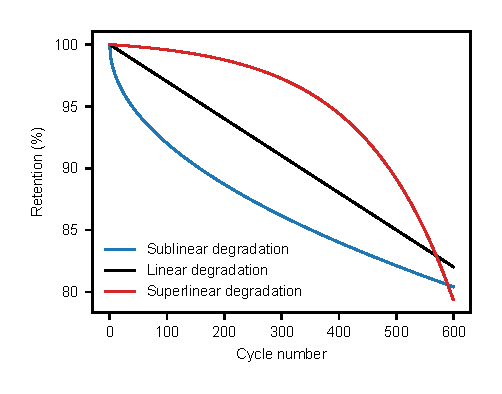
\includegraphics[scale=1]{figures/degradation_rates.eps}
\caption{Schematic of the three lithium-ion battery aging trajectories observed in the literature: sublinear, linear, and superlinear degradation (``knees''). Knees are incompatible with long battery lifetimes. Here, the $x$ axis is labeled ``cycle number'', although it could also represent equivalent cycles or similar; similarly, the $y$ axis is labeled ``retention'', although it could also represent absolute capacity, energy, or power. We use this convention (``retention vs. cycle number'') in conceptual figures throughout this work.}
\label{fig:degradation_shapes}
\end{figure}


In this review, we survey the literature and critically examine both experimental and modeling work on the subject of knees in lithium-ion battery aging. We first review methods to identify the knee point from an aging trajectory. We then identify six knee ``pathways'' from the literature, including lithium plating, cathode saturation, resistance growth, additive depletion, percolation-limited connectivity, and mechanical deformation. We also classify differences in experimentally observed knee behavior as either differences in design, differences in usage conditions, or cell-to-cell/testing variation. Finally, we discuss the implications of our review to both predicting and avoiding knees, and we suggest future work on this topic. This review can serve both academic and industrial efforts to understand and improve lithium-ion battery lifetime.

\section{Defining the knee point}

% \pbox{
% Key messages in my mind:
% \begin{itemize}
%     \item Knees seem easy to identify by eye, and have a nice mathematical description as the second derivative \cmark 
%     \item However noise makes this nontrivial (figure) \cmark
%     \item No formal definition (IEEE standard) \cmark
%     \item Briefly describe different methods
%         \subitem SG: We don't want this to take up too much space. If possible, a single plot with diagrams should suffice. \cmark
% \end{itemize}
% }

Mathematically, the knee is described as the point at which the degradation rate is changing fastest, i.e., the second derivative reaches some maximal value. IEEE Standard 485\texttrademark-2010  \cite{noauthor_ieee_2011} defines a (capacity) knee as a change to a stage of rapid decrease in capacity. However, this definition is qualitative and thus hard to practically apply: while the \textit{presence} of a knee is generally straightforward to identify, the \textit{location} of a knee is less so. 
Locating a knee by eye is seemingly straightforward for a single, smooth and ideal aging profile (e.g.,~the superlinear aging trend in Figure \ref{fig:degradation_shapes}). However, Figure \ref{fig:knee_definition3} demonstrates the problem of using a second derivative to identify the knee point with small amounts of noise (standard deviation of 0.05\% capacity, green) or with limited data points (blue) where the knee is artificially shifted later. The data is too discrete in either of these limiting cases. Furthermore, in deployed systems, varying duty cycles can effectively manifest as ``noise'' in estimates of capacity or energy.
Consequently, \textbf{CITE-Strange2021a} concluded that health metric profiles should be smoothed prior to knee identification, but aging trajectories with few data points remain problematic.

\begin{figure}[ht]
\centering
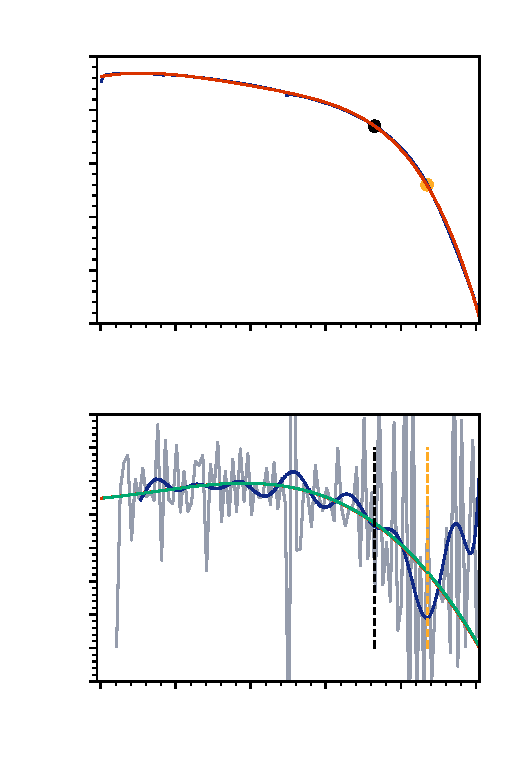
\includegraphics[scale=1]{figures/knee_definition.eps}
\caption{(a) Defining the knee point. The position of knee point as visually identified by an author (black point) differs from the mathematically defined knee point (yellow point). Data from batch 2, channel 12 cell from Severson et al.\cite{severson_data-driven_2019} The capacity is normalized by the nominal capacity of the cell. (b) Vulnerability of knee detection methods to noise.}
\label{fig:knee_definition3}
\end{figure}



\begin{figure}[h!tb]
\centering
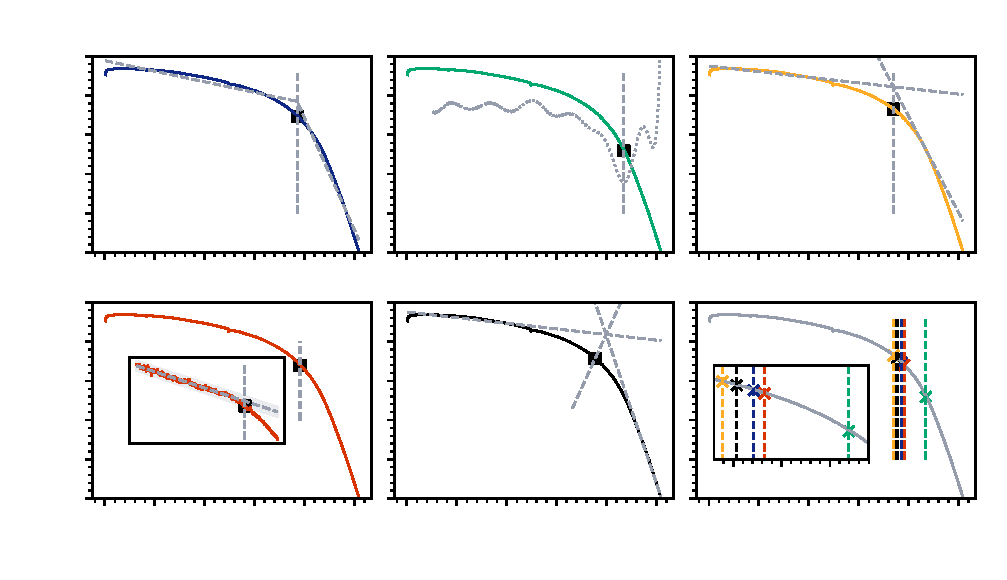
\includegraphics[scale=1]{figures/knee_identification_methods.eps}
\caption{Different knee identification methods exemplified on the cell from batch 2, channel 12 of Severson et al.\cite{severson_data-driven_2019}. The capacity is normalized by the nominal capacity of the cell. (a) Bacon-Watts \cite{fermin-cueto_identification_2020}, (b) Kneedle \cite{satopaa_finding_2011} (where the second derivative is also shown as a dotted gray line), (c) tangent-ratio from Diao et al.\cite{diao_algorithm_2019}, (d) Zhang et al.\cite{zhang_identifying_2020}, (e) Bisector from Greenbank and Howey(cite eventually). (f) Comparison of knee points as identified via these methods. 
(
WAIT UNTIL END TO ADD CITATIONS IN THE TEXT )}
\label{fig:knee_identification_methods}
\end{figure}

Several ``offline'' knee point identification methods have been proposed in the literature.
``Kneedle'' calculates the knee as the point of maximum curvature of the capacity curve \cite{satopaa_finding_2011}. The knee has also been calculated using the ``Bacon-Watts'' method for estimating the transition between two intersecting lines fitted to a capacity fade curve, a method which can also provide an estimate of the ``knee-onset'', the point where the aging trajectory is no longer linear \cite{fermin-cueto_identification_2020}. Other methods use tangential lines, such as the ``tangent-ratio'' (which defines the knee based on a tangent ratio at the inflection and maximum slope points of the capacity curve)\cite{diao_algorithm_2019} and the bisector method (which uses linear extrapolations of early and late life then an angle bisector identifies the knee as it intersects the capacity curve)\textbf{CITE-SAM\&David}. Finally, Zhang et al.\cite{zhang_accelerated_2019} proposed approximating early life with a linear regression, then defining a cell to have a knee if the capacity fell below a defined band about that regression line. The region is calculated using the variation in the height of a voltage peak; other methods do not require the use of voltage data. Of these five methods, the Bacon Watts and bisector methods are (arguably) the easiest to implement since they both avoid the use of derivatives and voltage data.

In Figure \ref{fig:knee_identification_methods}, we implemented and applied these methods to a single cell from Severson et al.\cite{severson_data-driven_2019}. All methods estimate the knee point at cycle numbers within a 20 cycle range (370--390 cycles) except the ``Kneedle'' method (435 cycles). These results held across most cells in the Severson et al.\cite{severson_data-driven_2019} dataset, suggesting that these methods are generally comparable for offline knee point estimation (see Supplementary Discussion 1 for details). We note that the ``Kneedle'' method most consistently estimated larger knee points than the other methods.

Finding the knee online, i.e., during use, is difficult because the end-of-life capacity profile is not known and because the discharging conditions are inconsistent. Transforming the offline methods into online methods is challenging since many of these methods require the entire aging trajectory for knee point estimation. However, the method of Zhang et al.\cite{zhang_accelerated_2019} can accommodate online knee point estimation since only the initial aging trajectory is required. Of course, the challenge of uncontrolled usage conditions is inherent to online state estimation; varying duty cycles in deployed systems could mask the knee.

% \gbox{
% Plan for the section (identify the references):
% \begin{itemize}
%     % \item The IEEE Standard 485\texttrademark-2010 \cite{noauthor_ieee_2011}\cmark 
%     % relates the “knee” with the transition to a stage of rapid decrease in capacity. This definition is qualitative not quantitative.

%     \item Very brief Overview of methods 

    
%     \begin{itemize}
%         % \item \cite{fermin-cueto_identification_2020}\cmark 
%         % , define the Knee based on Bacon Watts method for estimating the transition between two intersecting lines fitted to the capacity fade curve. Has the advantage of providing the concept of knee-onset.
%         % \item Kneedle  \cite{satopaa_finding_2011} \cmark 
%         % , define the knee as the point of maximum curvature of the capacity curve
%         % \item Diao \cite{diao_algorithm_2019}, define the knee as the intersection of two tangent lines to the capacity fade curve drawn at two significant points (an inflection point and the point of maximum slope changing ratio)
%         \item \cite{zhang_accelerated_2019} quantile, defined the knee-point as the intersection of two straight lines with different slopes and proposed an algorithm for online knee detection based on quantile regression (some parameter tuning is required). They fit a median regressor to the State of Health data and they define the knee as the first point at which the SOH data is outside a safety zone around the median regression line.
        
%         % \item {\tt Sam's Bissector}  
%     \end{itemize}
    
%     % These methods we implemented, and (empirically) tested in database of \cite{severson_data-driven_2019}. Noteworthy of remark is that the Kneedle's knee was always ahead of the Bacon Watts knee. In view of the a linear regression analysis between knee-point to EOL, 
    
%     % \item Present empirical analysis plot of linear regressions across datasets for knee-2-EoL (?) Supplementary material?
%     \end{itemize}
% }


%%%%%%%%%%%%%%%%%%%%%%%%%%%%%%%%%%%%%%%%%%%%%%%%%%%%
%%%%%%%%%%%%%%%%%%%%%%%%%%%%%%%%%%%%%%%%%%%%%%%%%%%%
%%%%%%%%%%%%%%%%%%%%%%%%%%%%%%%%%%%%%%%%%%%%%%%%%%%%
%%%%%%%%%%%%%%%%%%%%%%%%%%%%%%%%%%%%%%%%%%%%%%%%%%%%


\section{Pathways for knee points}

\pbox{
I still need to make a figure for all knee pathways
}

We surveyed the literature and identified six ``knee pathways''. These pathways are schematically illustrated in Figure X. Some of these pathways (e.g., lithium plating) have been extensively characterized and modeled, while others (e.g., percolation-limited knees) are merely hypotheses. Here, we critically examine the evidence for each pathway. For more extensively studied pathways such as lithium plating, we consider both \textit{modes}, defined as high-level changes in cell state, and \textit{mechanisms}, defined as the specific failure that leads to a change in cell state. For instance, active material loss is a degradation mode that can be caused by electrode delamination, one of several possible failure mechanisms for this degradation mode. Failure mechanisms are often challenging or impossible to pinpoint exactly or experimentally isolate, but failure modes are usually identifiable through common electrochemical measurements or characterization methods and can be considered to conceptually validate a proposed pathway.

We also consider the relationship between the observable state variables (i.e., capacity, energy, and power) and the mechanisms underlying their knee points. Figure \ref{fig:snowball_vs_hidden_vs_threshold} illustrates three underlying mechanisms that can lead to a knee. \textit{Snowball} mechanisms (Figure \ref{fig:snowball_vs_hidden_vs_threshold}a and \ref{fig:snowball_vs_hidden_vs_threshold}d) occur when the underlying state variable has a direct relationship with the observable state variable, but the underlying state variable is exponentially increasing. \textit{Hidden} mechanisms (Figure \ref{fig:snowball_vs_hidden_vs_threshold}b and \ref{fig:snowball_vs_hidden_vs_threshold}e) occur when the observable state variable, originally controlled by a slowly-increasing state variable, becomes dominated by a second rapidly-increasing state variable. Finally, \textit{threshold} mechanisms (Figure \ref{fig:snowball_vs_hidden_vs_threshold}c and \ref{fig:snowball_vs_hidden_vs_threshold}f) occur when the observable state variable changes when the underlying state variable reaches a threshold. Each of these underlying mechanisms has unique implications for detectability and prediction, a point we return to throughout this work.

\begin{figure}[h]
    \centering
    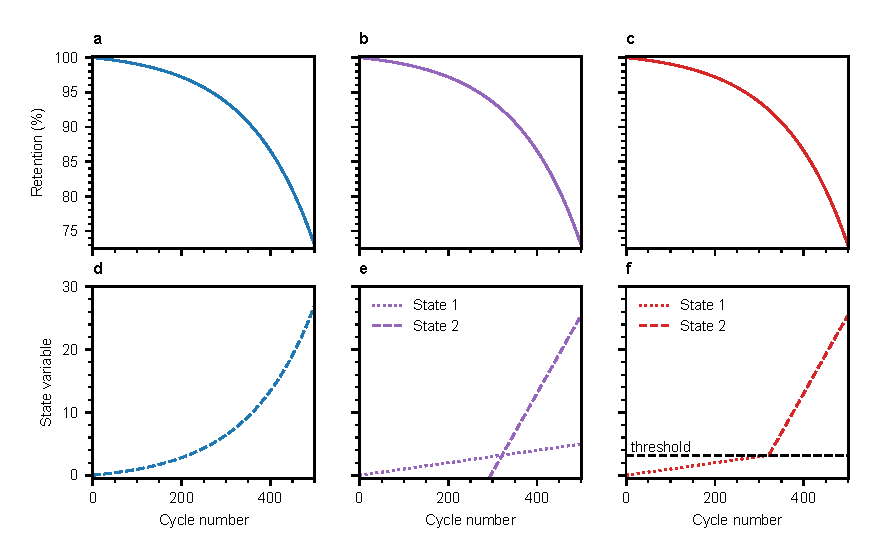
\includegraphics[scale=1]{figures/snowball_vs_hidden_mechanism.eps}
    \caption{Schematic of the three types of underlying mechanisms leading to a knee. In each case, the retention curve looks the same (a-c), but the underlying mechanism has a different functional form. (d) ``Snowball'' mechanism, in which the state variable is exponentially increasing. (e) ``Hidden'' mechanism, in which a slowly-increasing state variable is dominated by a rapidly-increasing state variable. (f) ``Threshold'' mechanism, in which a dramatic change in observable state is triggered by a state variable reaching a threshold.}
    \label{fig:snowball_vs_hidden_vs_threshold}
\end{figure}

\subsection{Lithium plating knees}

\pbox{
I still need to make a figure for all Li plating modes
}

Lithium plating occurs when lithium ions form metallic lithium on the surface of the electrode rather than intercalating into it. The plating reaction is favorable when the reaction potential of Li/Li$^+$ is greater than the equilibrium potential for other alternative reaction pathways for Li$^+$ (i.e., graphite intercalation).\cite{gao_interplay_2021} Plating can occur due to either ``thermodynamic plating'', or plating that occurs independent of the applied current, and ``kinetic plating'', or plating that only occurs if the applied current exceeds some value.  Furthermore, lithium plating can occur either reversibly or irreversibly. Irreversible plating leads to rapid loss of lithium inventory and has historically been considered to be a primary driver for capacity knees.

Generally, lithium plating on graphite follows heterogeneous nucleation and growth kinetics, in which rapid growth proceeds quickly after an initial nucleation phase.\cite{ely_heterogeneous_2013, pei_nanoscale_2017, gao_interplay_2021}
Thus, lithium plating can often be considered a ``snowballing'' knee (Figure \ref{fig:snowball_vs_hidden_vs_threshold}a and \ref{fig:snowball_vs_hidden_vs_threshold}d). However, some lithium plating pathways (e.g., lithium plating driven by active material loss from the negative electrode) will exhibit knees independent of 

Here, we discuss the mechanisms by which plating can lead to a knee (Figure X). We suggest Waldmann et al.\cite{waldmann_li_2018} and Gao et al.\cite{gao_interplay_2021} for comprehensive general overviews of lithium plating.

% Intro to plating
% \begin{itemize}
%     \item What is Li Plating?
%     \item Why does plating occur generally (V<Li)
%     equilibrium potential of the Li$\mathrm{^0}$/Li$\mathrm{^+}$ > everything else
%     \item Brief introduction to and definition of each plating pathway
%     \subitem Thermodynamic "non-current-induced"
%     \subitem Kinetic "current induced"
% \end{itemize}

\subsubsection{Thermodynamic lithium plating}

%- x$>0$
%- heterogeneous temperature
%- ${LAM}_{de}$NE

Thermodynamic lithium plating occurs whenever the lithium capacity during charging exceeds the negative electrode capacity, i.e., the negative electrode is unable to host all of the lithium from the positive electrode. Generally, the latter can be avoided in fresh cells by simply using a negative electrode to positive electrode capacity ratio (n:p ratio) greater than 1. However, if active material from the negative electrode is lost during aging, thermodynamic lithium plating will occur even in cells with excess negative electrode capacity.

\paragraph{Thermodynamic lithium plating in fresh cells}

While thermodynamic lithium plating in fresh cells can be easily avoided by proper cell design, this degradation mechanism is often exploited for scientific studies of lithium plating.
For instance, Deichmann et al.\cite{deichmann_investigating_2020} created cells with n:p ratios of 0.75 and 0.5 to intentionally deposit lithium metal on graphite electrodes. The authors identified a relationship between decreased n:p and capacity fade, which they attributed to high loss of lithium inventory using differential capacity analysis and SEM. In a creative study, Martin et al.\cite{martin_cycling_2020} used deposited lithium metal as a mechanism to store extra capacity, enabling the cell to occasionally discharge extra energy (i.e., when extra range is needed) without requiring a substantially larger negative electrode. This cell design used an n:p ratio of 0.6, where n:p is calculated using the lithium capacity of the conventional graphite. A high upper cutoff voltage during charging was used to intentionally plate lithium onto graphite; unsurprisingly, irreversible lithium plating was found to be the primary failure mechanism, with over 50\% capacity loss of lithium metal in two of the three electrolytes tested.

\paragraph{Thermodynamic lithium plating due to loss of active material}

Loss of active material --- specifically, loss of active material from the delithiated negative electrode ($\mathrm{LAM_{deNE}}$) --- during aging may result in thermodynamic lithium plating if the lithium capacity of the negative electrode becomes the limiting factor during charging. For instance, if the rate of $\mathrm{LAM_{deNE}}$ exceeds that of the loss of lithium inventory (LLI), the negative electrode will eventually be unable to accommodate all lithium during charging, which will lead to thermodynamic lithium plating and thus a knee. Dubarry et al.\cite{ansean_operando_2017, dubarry_durability_2018}(baure-synthetic-2019, dubarry-big-2020) extensively explored this scenario, considering different ratios of $\mathrm{LAM_{deNE}}$ to LLI as well as different extents of reversible and irreversible plating (Figure \ref{fig:thermo_plating}). This case is a prototypical case of a hidden state (i.e., loss of active negative electrode material) causing a knee.

\begin{figure}[ht]
    \centering
    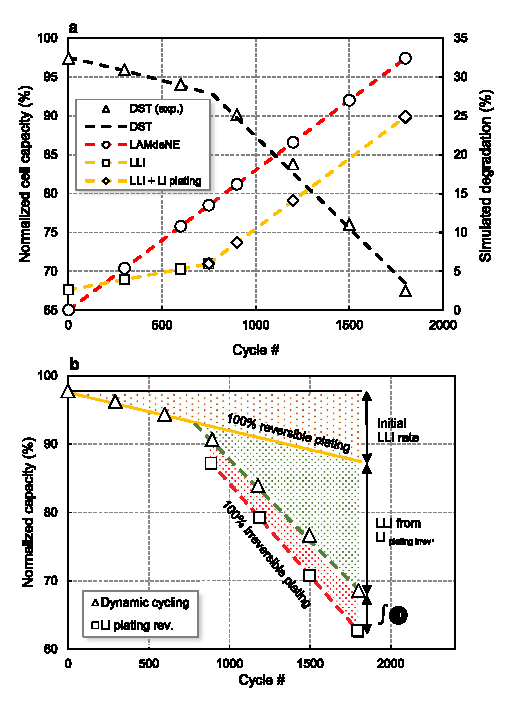
\includegraphics[scale=1]{figures/thermo_plating_dubarry.eps}
    \caption{Thermodynamic lithium plating driven by loss of active negative electrode material. (a) Evolution of aging parameters with cycling of cell degradation. The left axis shows the experimental normalized cell capacity (triangle markers), and the dashed black line shows the results of cell capacity simulations with the calculated aging modes. The right axis shows the evolution of the degradation induced by the calculated aging modes (markers and dashed lines) with cycling. Note that $\mathrm{LAM_{deNE}}$ increases linearly, and at a rate higher than LLI.
    (b) Capacity vs. cycle number at low rate (C/25), depicting the contributions to the total capacity fade as a function of cycle number.
    Adapted from Figures 7 and 8 of Anse\'an et al.\cite{ansean_operando_2017}}
    \label{fig:thermo_plating}
\end{figure}

Various degradation mechanisms can lead to $\mathrm{LAM_{deNE}}$, which occurs when active sites lose either ionic or electronic connectivity with the electrode.
Often, several of these mechanisms can occur in parallel, leading to a snowball effect where loss of active material due to one mechanism may result in further stress on the remaining active sites, accelerating degradation via thermodynamic lithium plating.
Electrode sites can lose ionic connection via electrolyte dry-out, which may be driven by gas generation during cycling.\cite{mao_calendar_2017, kupper_end--life_2018}
Electrode sites can lose electronic connection via delamination\cite{cannarella_stress_2014, willenberg_high-precision_2020}(liu, somerville), particularly for cells with low external pressure\cite{cannarella_stress_2014}. Particle cracking is another mechanism for electronic disconnection of active sites, although cracking is not expected to occur appreciably in graphite particles.(Takahashi-examination)

An additional $\mathrm{LAM_{deNE}}$ mechanism is the growth of thick layers ($1-10 \mathrm{\mu m}$ on the surface of the negative electrode, sometimes termed ``covering layers''\cite{lewerenz_post-mortem_2017, lewerenz_systematic_2017, willenberg_development_2020}.
Surface layer growth-driven $\mathrm{LAM_{deNE}}$ may impede lithium-ion transport into the negative electrode during charging, effectively isolating portions of the electrode and resulting in an apparent loss of active material. This surface layer is commonly observed in cells with knees and is often attributed to manganese or iron dissolution from the cathode and electrolyte salt decomposition, \cite{lewerenz_post-mortem_2017,lewerenz_systematic_2017,zhu_investigation_2021,stiaszny_electrochemical_2014,rahe_nanoscale_2019,keil_linear_2019,sarasketa-zabala_understanding_2015, willenberg_high-precision_2020} but the root cause has not been definitively identified. Peculiarly, the size of these layers (microns) is much larger than typical reported SEI thicknesses (nanometers)\cite{peled_reviewsei_2017}. Lewerenz et al.\cite{lewerenz_post-mortem_2017,lewerenz_systematic_2017} thoroughly documented surface layer growth, finding that increasing C-rate and larger depth-of-discharge could lead to earlier onset of a knee. Earlier knee onsets was correlated with the presence of a thick surface layer on cells that contained knees; cells without knees also contained obvious surface layers, but with lower surface coverage and less thickness. These surface layers sometimes seem to lead directly to localized lithium plating due to the lack of active sites available for lithium insertion, with lithium observed on top of the layer.\cite{zhu_investigation_2021}
Further investigation of these surface layers is needed to understand this seemingly ubiquitous mechanism for loss of active negative electrode material.

\begin{figure}[ht]
\centering
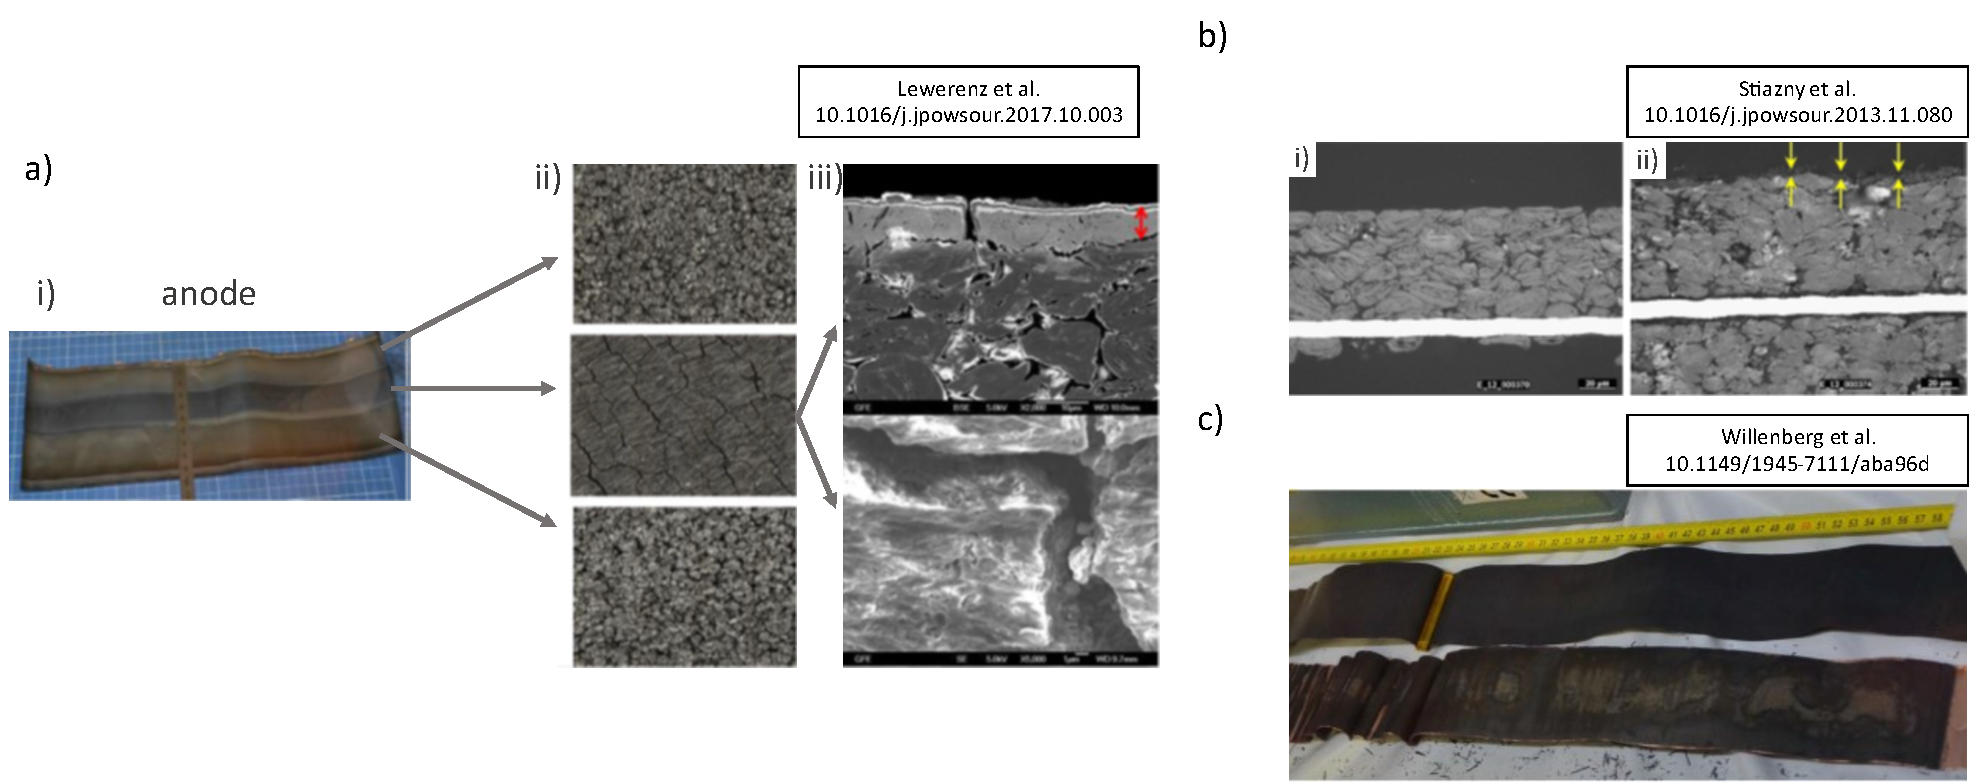
\includegraphics[scale = 0.5]{figures/CoveringLayers.pdf}
\caption{``Covering layers'' found via post-mortem analysis in cells with knees. a) A covering layer in the middle of the anode of an unwound cylindrical cell, along with laser microscope images of top, middle and bottom sections and SEM images of the middle section with a covering layer. Reproduced with permission from Lewerenz et al. \cite{lewerenz_post-mortem_2017} Copyright 2017, Elsevier. b) Covering layer in the middle of the anode of an unwound cylindrical cell. The red arrow corresponds to a thickness of $10 \mathrm{\mu m}$. CC-By Willenberg et al. \cite{willenberg_development_2020}. c) SEM cross-sections of new and aged electrodes with a visible covering layer. Reproduced with permission from Stiaszny et al. \cite{stiaszny_electrochemical_2014} Copyright 2014, Elsevier.}
\label{fig:covering_layers}
\end{figure}

\subsubsection{Kinetic lithium plating}
%- this is when transient effects cause plating
%- Low T -> Low D -> High Surface x -> ${eta}_{s}$<0
%- Low OCV + High ${eta}_{op}$ -> ${eta}_{n}$<Li
%- High σ -> Low ρ -> High Surface x -> ${eta}_{s}$<0
%- SEI -> Low ρ -> High Surface x ->${eta}_{s}$<0

``Kinetic'' lithium plating occurs when excessive transport or reaction overpotentials cause the local electrode potential to drop below that of Li/Li$\mathrm{^+}$.
In other words, kinetic lithium plating occurs at conditions when the plating could otherwise be mitigated by lithiating the graphite at a sufficiently low current. As Gao et al.\cite{gao_interplay_2021} describe, salt depletion in the electrolyte or surface crowding in the graphite at the graphite surface further favor lithium plating over intercalation. While kinetic lithium plating can occur via similar mechanisms to thermodynamic lithium plating, the dynamic nature of this process introduces additional avenues for lithium plating knees to occur.

\paragraph{Kinetic lithium plating in fresh cells}
Kinetic lithium plating can be driven by a wide range of cell designs and usage conditions; the prototypical use case leading to lithium plating is high charging rates at low temperature \cite{waldmann_temperature_2014, petzl_lithium_2015}. Waldmann et al.\cite{waldmann_temperature_2014} observed an increase in the rate of aging with a decrease in temperature below 25$^{\circ}$C, attributing the increased aging rate to lithium plating via dissections. Low temperatures increase both the transport overpotentials for lithium ions within the electrolyte and electrode and the reaction overpotential for litihum intercalation. Note that ``high'' charging rate or ``low'' temperature do not have consistent quantitative definitions, as plating will occur whenever the local potential exceeds the energy barrier for lithium nucleation. Thus, plating may be observed even at ``standard'' test conditions, such as 1C constant-current charging near room temperature \cite{waldmann_optimization_2015,burns_-situ_2015}. Increasing temperature and improved cell design (i.e., thinnener electrodes) may allow for much more rapid charging before lithium plating and knees are observed; Lewerenz et al.\cite{lewerenz_systematic_2017} cycled cells at rates up to 8C, observing no knees at rates as high as 4C, though microstructural evidence of plating was found even at 1C. The onset of lithium plating is also sensitive to the charging protocol, with many studies demonstrating that informed design of charging protocols can substantially extend cell lifetime by preventing direct lithium plating.\cite{waldmann_optimization_2015,schindler_fast_2018}. Optimizing electrode architectures to improve electrolyte transport kinetics is a further path forward to increase charging currents without lithium plating \cite{usseglio-viretta_enabling_2020} (nemani design)

Exterior mechanical stress may also lead to kinetic lithium plating, as applied stress can compress the electrode or separator. This compression locally decreases the porosity of the electrodes, reducing the diffusivity of electrolyte and thus increasing the local polarization and causing lithium plating. A direct test of this mechanism was conducted by Liu and Arnold\cite{liu_effects_2020}, who demonstrated that localized lithium plating could be induced in densified regions of the separator. Bach et al.\cite{bach_nonlinear_2016} applied a hose clamp around the circumference of an 18650 cell, and a post-test teardown clearly showed lithium plating localized to the regions of the electrodes that were under compressive stress. Coin cell and pouch cells also show similar results.\cite{liu_size_2018, fuchs_post-mortem_2019, okasinski_situ_2020}

\paragraph{Kinetic lithium plating due to loss of active material}

\paragraph{Kinetic lithium plating due to pore clogging}
As SEI grows, it precipitates mainly in the pores of the anode, decreasing the volume fraction of the electrolyte in the anode \cite{sikha_effect_2004}. The decreased volume fraction increases the electrolyte transport overpotentials, which can ultimately lead to lithium plating. The plated lithium, which has a much lower density than intercalated lithium\cite{yang_modeling_2017}, further decreases the porous volume fraction, creating a positive feedback loop for additional lithium plating\cite{yang_modeling_2017}. Several authors have noted that a critical porosity exists around 0.05, beyond which a knee occurs \cite{yang_modeling_2017, muller_model-based_2019}. This effect has also been modeled by simply decreasing the diffusion coefficient as a function of cycle number \cite{keil_electrochemical_2020}. One proposed countermeasure for this issue is to use a graded or stepped porosity profile through the thickness of the negative electrode. Since most pore clogging occurs near the separator, having a higher porosity near the separator and a lower porosity near the current collector can slow the onset of the knee caused by pore clogging \cite{muller_model-based_2019}.
While this 

\begin{figure}[h]
    \centering
    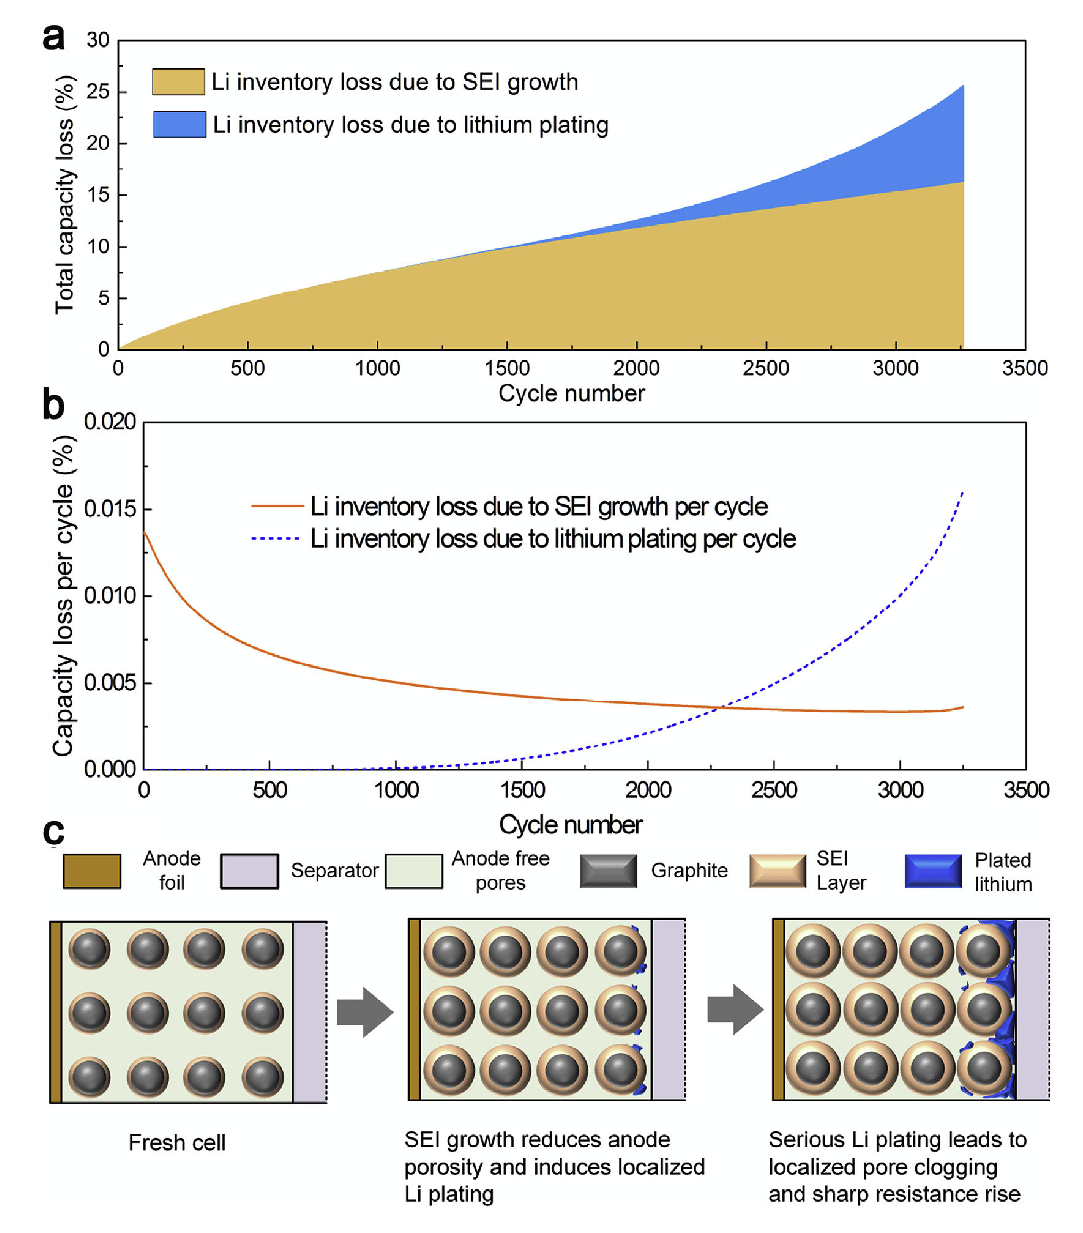
\includegraphics[scale=0.9]{figures/li_plating_porosity_yang.eps}
    \caption{Kinetic lithium plating due to pore clogging. (a) Lithium inventory loss contributed by SEI growth and lithium plating, respectively. (b) Lithium inventory loss per cycle contributed by SEI growth and lithium plating, respectively. The ``snowballing'' growth of lithium plating occurs due to the accelerating decrease in porosity, which creates high transport overpotentials in the electrolyte and drives additional plating. (c) Schematic illustration of pore clogging driven initially by SEI growth and then by plating. Adapted from Figure 8 of Yang et al.\cite{yang_modeling_2017}}
    \label{fig:pore_clogging}
\end{figure}

\paragraph{Heterogeneity-based pathways}

\begin{figure}[ht]
\centering
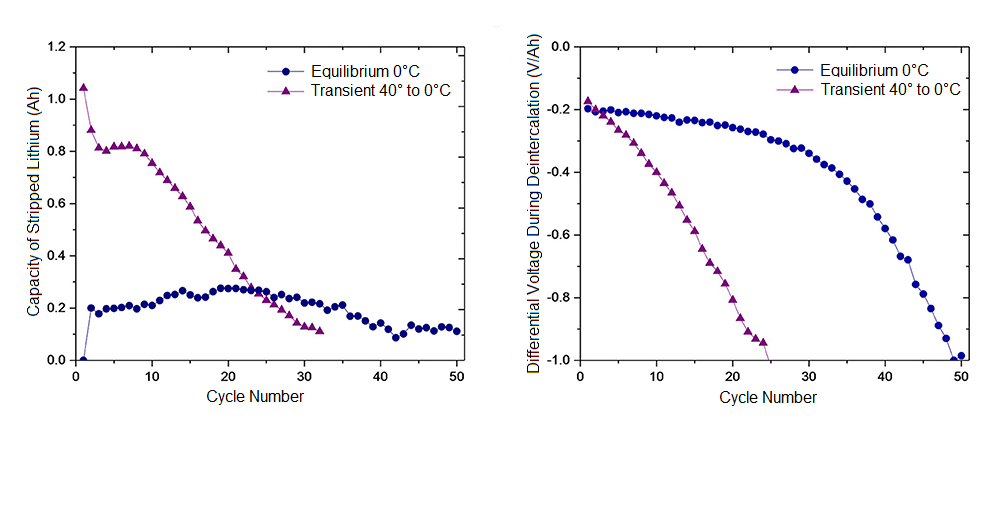
\includegraphics[scale = 1]{images/Capacity & Diff Voltage.png}
\caption{Capacity and differential vapacity vs cycle number.
\textbf{More info needed here.
Also is differential voltage needed?}
Figure obtained from X et al.[]
}
\label{fig:CapDiffCapCycle}
\end{figure}

Apart from the main mechanisms causing knees due to plating, few other causes are based on substantial and mild temporally thermal transient conditions lead to a rapid capacity fade in cells when compared with cells at a fixed equilibrium temperature. Temporal transient thermal gradients (40 \degree C to 0 \degree C), or temperature heterogeneity, can contribute to Li ions being plated as Li instead of intercalating, which accelerates capacity fade over subsequent cycles causing knees and ultimately resulting in jellyroll collapse.

Equilibrium cells at 40 \degree C, 20 \degree C, 0\degree C and transient cells (40\degree C to 0 \degree C and 10 \degree C to 0 \degree C) are tested for understanding of the thermo-electrochemical coupling across different temperature (Carter 2019). Differential voltage from charging shows evidence for plating and discharging cycle showcases the degradation modes. Equilibrium cells at 40 \degree C and 20 \degree C show minimal degradation while equilibrium cell at 0 \degree C has initial minimal degradation, then a gradual decay midway. On the contrary, transient 10 \degree C to 0 \degree C cell and 40 \degree C to 0 \degree C cell show degradation at earlier cycles (8 and 5 respectively) (Carter, 2019). Transient 40 \degree C to 0 \degree C cell demonstrates high lithium stripping during initial discharge cycles due to thermal transient induced plating causing increase in anode thickness, pressure buildup in jelly role and capacity loss. The decrease in differential voltage for transient cells immediately with the start of the cycle shows the degradation evidence by lithium plating.  Figure 7 highlights the difference between the 0 \degree C and Transient 40 \degree C to 0 \degree C jellyroll collapsing behaviors. Primary reason for degradation is jellyroll collapse for 0 \degree C cell while the rapid lithium plating followed by jellyroll collapse causes capacity fade knee point in Transient 40 \degree C to 0 \degree C cell. 

\subsection{Cathode saturation}

\pbox{Tino: Let's work on this section together}

Lin et al.~\cite{lin_comprehensive_2013} proposed a different mechanism for knee caused by loss of active material. In their model, SEI growth leads to loss of lithium inventory and mechanical effects in the cathode lead to LAM. This causes the cathode utilization to increase and shift to a steeper open-circuit potential, which reduces the capacity between voltage limits. This mechanism produces a non-linear capacity fade (knee), due to the non-linearity of the open-circuit potential, despite linear LAM and self-limiting SEI formation. The knee point occurs when loss of active material outpaces loss of lithium inventory, as suggested by Dubarry et al.\cite{dubarry_durability_2018}.

\subsection{Resistance growth knees}

Increasing resistance during cycling intuitively leads to a decrease of cell power, regardless of the thermodynamic capacity of the battery, due to increased overpotential. Additionally, increasing resistance may also lead to the onset of a knee in the accessible capacity. This is intuitive at high currents, when even a high-performing cell may become rate limited and reach a voltage cutoff before the majority of lithium has been shuttled across the separator. However, during aging, this rate limitation may occur at much lower than expected C-rates, and appear as a knee in the plots of both power and capacity versus cycles. This behavior was thoroughly studied by Ma et al \cite{ma_editors_2019} using lab-made 230mAh NMC532/graphite pouch cells, varying the upper cutoff potential, discharging rate, electrolyte composition, and type of graphite. Careful study using impedance measurements, both of the full cells as well as symmetric coin cells of the positive and negative electrodes, was used to isolate the loss of performance to a dramatic increase of the cathode impedance during aging. This DC resistance growth was attributed to electrolyte oxidation at the positive electrode, which occurred more quickly at higher upper cutoff potentials and was also dependent on the electrolyte composition. One practical consideration from the work is that periodic high rate discharge tests exhibit resistance growth induced knee onset earlier than low rate discharge tests, and thus serve as an early indication of future cell knee onset at lower rates. Similar onset of a capacity knee due to the selection of the electrolyte composition was previously observed by Li et al as well \cite{li_methyl_2018}. 

A simple model illustrating knee onset due to ohmic resistance growth during cycling, inspired by Ma et al \cite{ma_editors_2019} and Mandli et al \cite{mandli_analysis_2019}, is shown in detail in Figure \ref{fig:dcr_knee}. The model assumes a constant increase of the resistance of 0.2 milliohms per cycle during cycling of a 3 Ah NMC/Gr lithium-ion battery; the increase of resistance leads to a linear increase in the ohmic overpotential at every cycle (Fig. \ref{fig:dcr_knee}a). This linear increase in ohmic potential then leads to a downshift of the voltage-capacity curve; to demonstrate the impact of increasing resistance on measured capacity, energy, and power retention due to this downshift in a 'real' cell, voltage-capacity and voltage-energy relationships are used from experimental NMC/Gr cell data recorded at beginning-of-life from Preger et al \textbf{[Preger, added to zotero]} (Fig. \ref{fig:dcr_knee}b). Fig. \ref{fig:dcr_knee}c,d show the impacts of this downshift on the voltage-capacity curve at lower voltage cutoffs of 2 V and 2.8 V; for the 1C case (Fig. \ref{fig:dcr_knee}c) both the 2 V and 2.8 V cutoffs occur on the nonlinear portion of the voltage capacity curve at the beginning of life. But as the cell ages and the resistance increases, the voltage curve shifts down, leading to the 2.8 V cutoff being reached by the linear portion of the voltage-capacity relationship, causing more rapid fade in the measured capacity than was initially observed. The impact of the resistance growth on the measured capacity (Fig. \ref{fig:dcr_knee}e), energy (Fig. \ref{fig:dcr_knee}f), and power (Fig. \ref{fig:dcr_knee}g) delivered during the discharge over the cell lifetime varies depending on the C-rate and the lower voltage cutoff. The unexpected power retention trends versus cycle number, C-rate, and lower voltage cutoff illustrate some limitations of such a simplistic model for cell resistance, as other non-linear cell polarization behaviors such as charge transfer polarization and cell heating during increased current should also impact the voltage response of the cell in addition to the ohmic effects modeled here. The shift of the lower voltage cutoff from the high slope portion of the voltage-capacity relationship to a lower slope portion of the voltage-capacity relationship may also occur due to a stoichiometric decrease of lithium available to cycle, as explored by Mandli et al \cite{mandli_analysis_2019}, or a stoichiometric shifting of lithium to one electrode preferentially during aging due to uneven loss of active material across the two electrodes of the cell \cite{lin_comprehensive_2013}. Cell chemistry may have dramatic impacts on the observed trends; the flatter linear portion of the voltage-capacity relationship of an LFP/Gr cell would result in a much sharper knee than the NMC/Gr voltage-capacity relationship used here. All things considered, the combined impacts of resistance growth, lithium loss, and active material losses on the measured voltage response of any lithium-ion battery may explain many observed knee behaviors in cells that are not experiencing sudden failure due to lithium-plating induced shorting, electrode delamination, or other types of readily observable failure.

\begin{figure}[ht]
\centering
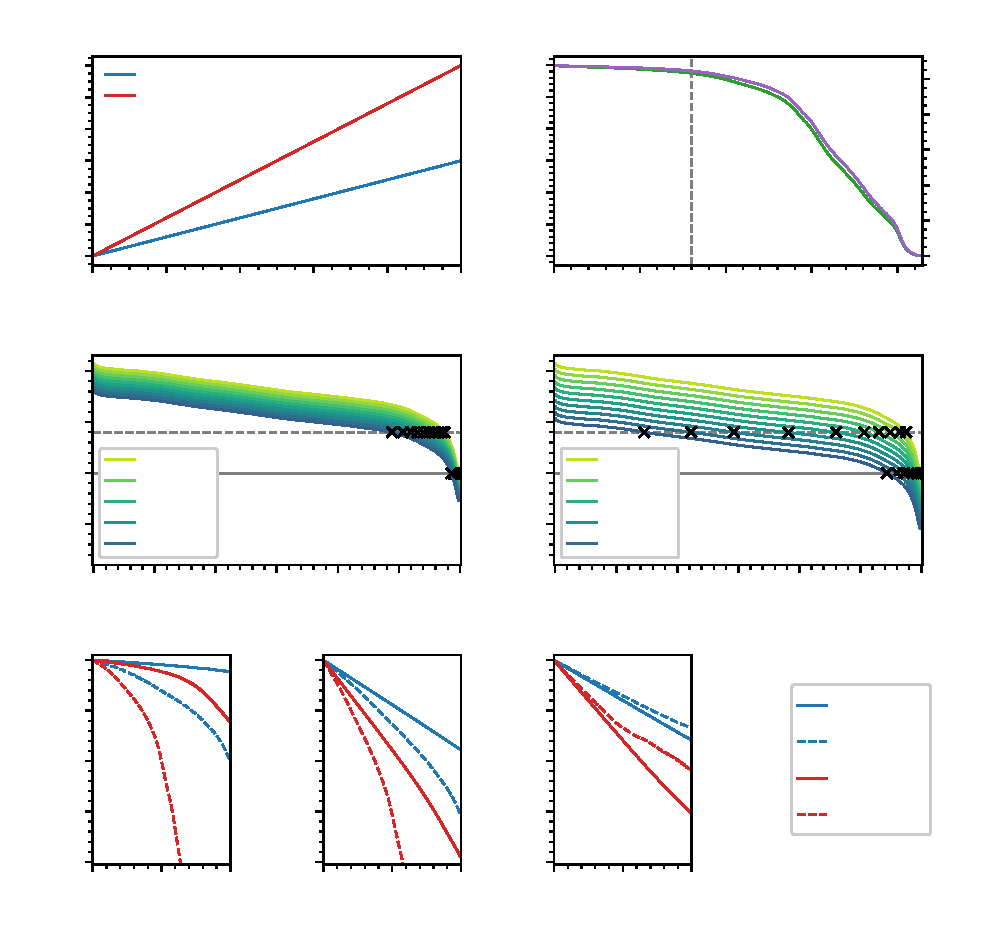
\includegraphics[scale = 1]{figures/dcr_growth_knee_2.eps}
\caption{Simple model illustrating ``pseudo-knees'' due to resistance growth; we use the term ``pseudo-knees'' here since the knee location is a function of rate and lower cutoff voltage. Inspired by Figure 16 of Ma et al.\cite{ma_editors_2019} and Mandli et al.\cite{mandli_analysis_2019}. (a) Assumed overpotential growth vs. cycle number for a 1C and 2C discharge. The assumed resistance growth rate is 0.2 m$\Omega$/cycle. (b) Discharge capacity and energy vs. the minimum discharge voltage for an example NMC/graphite cell. Data obtained from Preger et al.\cite{preger_degradation_2020} (c, d) Voltage vs. capacity as a function of cycle number for the (c) 1C discharge and (d) 2C discharge cases. The final discharge capacity for each cycle is denoted by a marker. (e--g) (e) Capacity, (f) energy, and (g) power retention vs. cycle number as a function of discharge current and the minimum voltage.
}
\label{fig:dcr_knee}
\end{figure}

This observation is supported by the fact that many aging studies have shown that capacity knee onset is nearly always correlated to the onset of rapid resistance growth, across different cell chemistries, architectures, and test protocols. The relative capacity and resistance at the knee onset point from several studies that reported both capacity fade and resistance growth are reported in Table \ref{tab:dcr_growth_papers}. Of all these aging studies, cells with capacity knees always displayed resistance elbows, and with the exception of the work by Martinez-Laserna et al \cite{martinez-laserna_technical_2018}, the reverse is also true. One assumption used in the model shown in Fig. \ref{fig:dcr_knee} but not reflected in these results is that linear resistance growth continues after knee onset; in much of the experimental work, regardless of the remaining capacity or relative resistance growth at knee onset, the previously linear resistance growth suddenly accelerates, leading to a resistance elbow as well. This is likely because many of the resistance growth and capacity fade mechanisms are intertwined. For instance, SEI growth causes both an increase in cell resistance as well as a decrease in available lithium, while loss of electrode active material may cause stoichiometric shifts of lithium while also decreasing available surface area for electrode-electrolyte reactions and thereby increasing cell resistance as well.

\hfil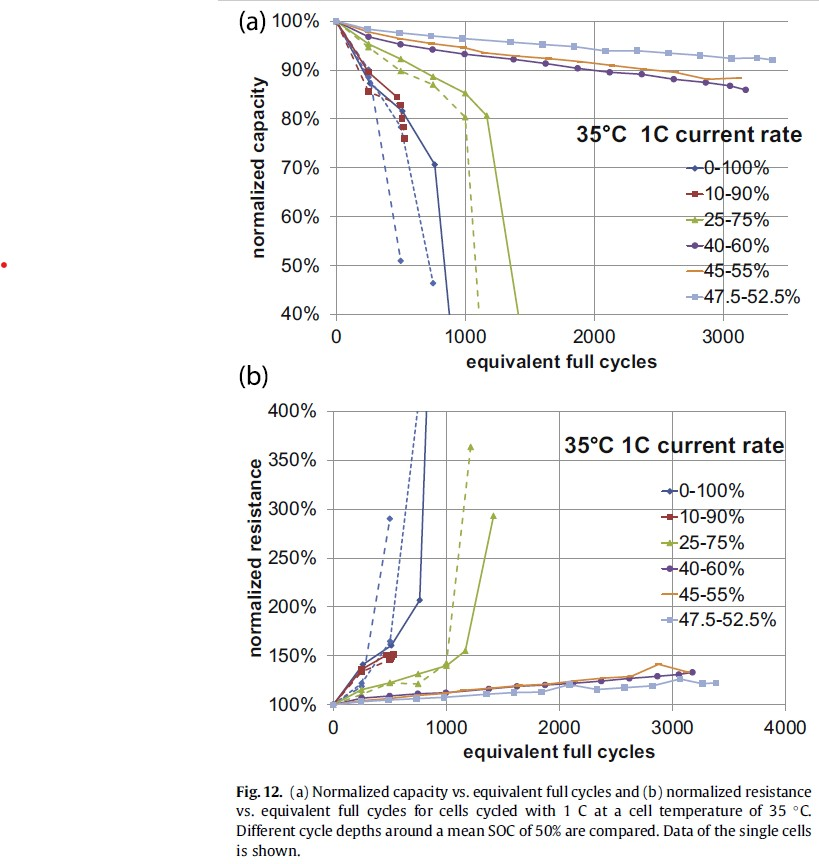
\includegraphics[scale=1]{images/Ecker_2014_fig12.jpg}

\begin{table}[!ht]
    \centering
    \begin{tabular}{||c||c|c|c|c||}
        \hline
        Ref. & Multiple test conditions? & Test replicates? & Rel. capacity at knee onset & Rel. resistance at elbow onset \\
        \hline
        \cite{ecker_calendar_2014} & Yes & No & 80\% & 150\% \\
        \cite{rahe_nanoscale_2019} & No & No & 90\% & 160\% \\
        \cite{willenberg_development_2020} & No & Yes & 90\% & 120\% \\
        \cite{broussely_main_2005} & No & Yes & 70\% & 200\% \\
        \cite{schuster_nonlinear_2015} & Yes & No & 80\% & 300\% \\
        \cite{lewerenz_systematic_2017, lewerenz_post-mortem_2017} & Yes & Yes & 80\% & 110\% \\
        \cite{martinez-laserna_technical_2018} & Yes & No &  85\% & 170\% \\
        \cite{braco_experimental_2020} & No & Yes & 70\% & 200 \% \\
        \cite{frisco_understanding_2016} & No & No & 80\% & 200\% \\
        \cite{klett_non-uniform_2014} & No & No & 80\% & 110\% \\
        \cite{pfrang_long-term_2018} & No & Yes & 75\% & 130\% \\
        \cite{wunsch_investigation_2019} & Yes & No & 95\% & 100\% \\
        \hline
    \end{tabular}
    \caption{Summary of studies reporting both capacity and resistance over cell lifetime with capacity knees and/or resistance elbows. All studies measure resistance using a direct-current pulse except for Schuster et al. \cite{schuster_nonlinear_2015}, which uses EIS. Relative capacity and resistance values at capacity knee/resistance elbow onset are estimated either from a single measurement or roughly averaged from several measurements.}
    \label{tab:dcr_growth_papers}
\end{table}



\subsection{Additive depletion knees}

Electrolyte additives have an disproportionate effect on lifetime relative to their presence in a cell; small quantities of electrolyte additives can often delay the occurrence of the knee by many cycles\cite{ma_editors_2019} (also cite Li 2017 comparison). Additive chemistry is complex; for instance, Burns et al.\cite{burns_predicting_2013} showed how electrolyte performance often improves with the number of additives used. Additives can influence the onset of lithium plating knees via various mechanisms (e.g., electrolyte transport properties, SEI growth rate, etc) and resistance growth knees by controlling the rate of resistance growth\cite{ma_editors_2019}. However, the \textit{depletion} of electrolyte additives is another demonstrated knee pathway. Here, we discuss perhaps the most widely studied additive depletion knee mechanism: fluoroethylene carbonate (FEC) depletion in silicon-containing cells.

FEC has been shown to substantially improve the capacity retention of silicon electrodes.(cite Choi 2006, Etacheri 2012)
Among standard electrolyte components, FEC preferentially reacts at the surface of silicon particles; in fact, the rate of FEC consumption on silicon is 10x that of graphite, in part due to its large volume expansion (around 300\%).\cite{wetjen_differentiating_2017}
Petibon et al.\cite{petibon_studies_2016},
Jung et al.\cite{jung_consumption_2016},
and Wetjen et al.\cite{wetjen_differentiating_2017}
performed comprehensive studies of Si-containing full cells with FEC-containing electrolytes and commercially-representative volumes,
conclusively demonstrating that a knee occurs when FEC is depleted from the electrolyte.
Figure \ref{fig:fec_knee} displays key results from Petibon et al.\cite{petibon_studies_2016} and
Jung et al.\cite{jung_consumption_2016}, in which the dependence of the knee on FEC concentration was confirmed via destructive measurements of FEC concentration vs. cycle number\cite{petibon_studies_2016} and cycling cells with increasing initial FEC concentration\cite{jung_consumption_2016}.
Louli et al.\cite{louli_operando_2019} also corroborated these findings.
Earlier studies of the use of FEC in high-Si cells (cite Choi 2006, Etacheri 2012) did not observe this knee mechanism due to their use of high electrolyte volumes, which provided a large reservoir of FEC.
Other electrolyte components (namely, linear carbonates) are consumed only after the knee, since FEC can no longer be preferentially consumed\cite{petibon_studies_2016}; the cell polarization increases substantially after the knee\cite{petibon_studies_2016, jung_consumption_2016, wetjen_differentiating_2017}, possibly due to high reaction overpotential from reactions of silicon with these nonpreferred electrolyte components.
Note that this mechanism is exacerbated by high upper cutoff voltages \cite{petibon_studies_2016}, higher cycling rates (presumably due to more mechanical damage to the SEI layer) \cite{petibon_studies_2016}, and (presumably) high temperatures (due to higher SEI growth rates).

\begin{figure}[ht]
\centering
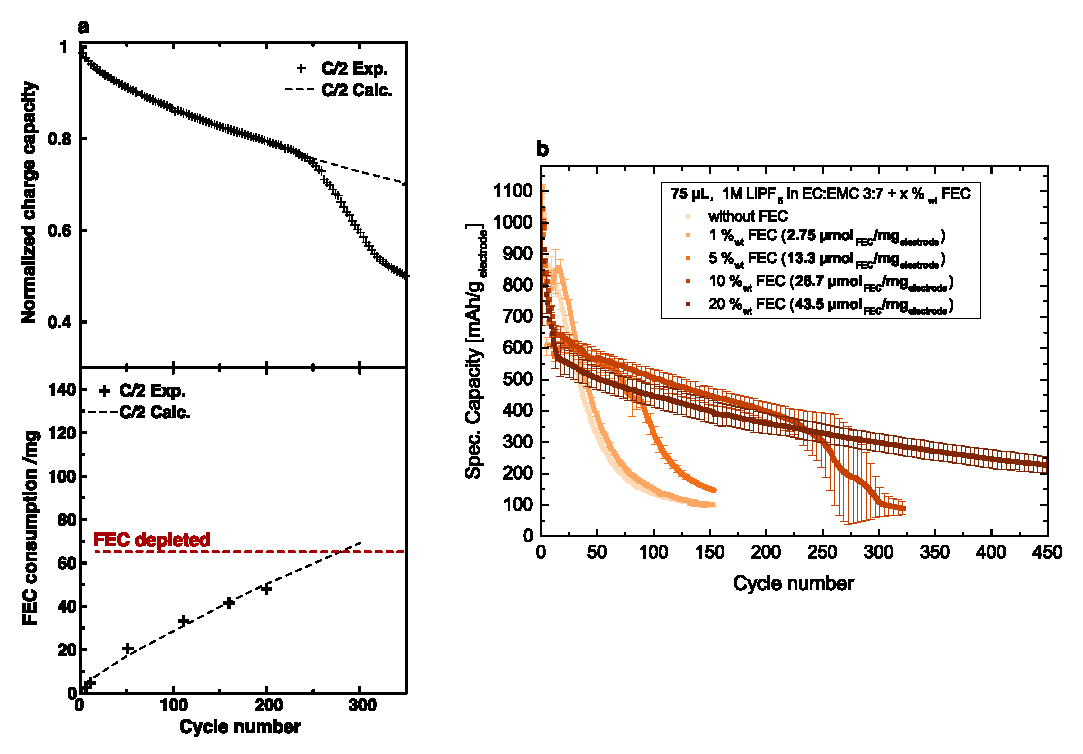
\includegraphics[scale = 0.9]{figures/fec_depletion.eps}
\caption{Additive depletion knees.
(a) The capacity retention of a full cell with 15\% Si in the negative electrode exhibits a knee at around 250 cycles, the same point at which the FEC is depleted from the electrolyte (from destructive gas chromatography-mass spectrometry measurements of FEC concentration). Adapted from Figure 8 of Petibon et al.\cite{petibon_studies_2016}
(b) In half cells with 100\% Si negative electrodes, the cycle number of the knee increases with the FEC concentration in the electrolyte. Adapted from Figure 1 of Jung et al.\cite{jung_consumption_2016}}
\label{fig:fec_knee}
\end{figure}

This knee pathway has a number of interesting implications.
First, since laboratory-built cells are often filled with high electrolyte volumes, knee mechanisms that are not present in lab testing may manifest in more commercially representative form factors.
As Wetjen et al.\cite{wetjen_differentiating_2017} emphasize,
maintaining representative electrolyte volumes in lab-scale cells is critical for accurately capturing this knee pathway in production-scale cells.
Second, nominally identical cells, cycled identically, but with different initial FEC concentrations exhibited minute electrochemical differences before the knee.\cite{jung_consumption_2016}
Theoretically, only the FEC consumed in a given cycle manifests in the electrochemical signals from cycling (e.g., differential capacity or differnetial voltage analysis); the excess FEC is not electrochemically detectable as it does not participate in reactions with the electrode.
Since the \emph{remaining} FEC amount is the main determinant of cycle life in these cells, the knee point of cells exhibiting this mechanism is not predictable via standard electrochemical signals.
An interesting proposal for future work is to evaluate other nondestructive probes (e.g., acoustic signals\cite{knehr_understanding_2018}) that may be sensitive to FEC concentration in the electrolyte.

\subsection{Percolation-limited connectivity knees}

Percolation theory \cite{essam_percolation_1980, stauffer_introduction_1994} is commonly used to describe statistical properties of clusters that are geometrically connected in porous media, including porous electrodes used in modern lithium-ion batteries\cite{ferguson_nonequilibrium_2012}. In a porous medium described by percolation theory, there exists a critical material parameter, above which the probability of a spanning cluster being formed tends towards one and below which this probability tends towards zero.\cite{ferguson_nonequilibrium_2012} In many percolating systems, this probability is highly sensitive to the value of the critical material parameter. For lithium-ion batteries, percolation theory can be used to describe both the ionic conductivity of the liquid electrolyte that fills the porous electrode and the electronic conductivity of the network of conductive additives. In battery modeling and experimentation, the electrode is often implicitly assumed to be sufficiently porous for the liquid electrolyte to completely percolate it. On the other hand, much effort has been spent on elucidating how the volume fraction of conductive additives may or may not give rise to a percolating electrically conducting network~\cite{li_effects_2015, cerbelaud_understanding_2015, guzman_improved_2017} (also cite Chen et al.), which is especially important for ensuring electronic conduction is not rate-limiting in electrically insulating active materials such as lithium iron phosphate.\cite{li_effects_2015, guzman_improved_2017}

Kupper et al.\cite{kupper_end--life_2018} examined the commonly held assumption that the liquid electrolyte always percolates the porous electrode by adding a degradation mechanism that accounts for electrolyte dry-out, which results in loss of ionic contact between the active material and electrolyte and thus the subsequent loss of active material. In doing so, their model predicts ``sudden death'' of the cell capacity, which is equivalent to a knee. In this proposed electrolyte dry-out mechanism, they first define two new electrode descriptors: ``activity'', $a$, and ``saturation'', $s$, given by $a = \frac{\varepsilon_{\text{LiC}_6}}{\varepsilon_{\text{LiC}_6,\text{inactive}}+\varepsilon_{\text{LiC}_6}}$ and $s = \frac{\varepsilon_\text{elyt}}{\varepsilon_\text{elyt}+\varepsilon_\text{gas}}$, respectively. In these equations, $\varepsilon$ is the volume fraction of the active graphite ($\varepsilon_{\text{LiC}_6}$), inactive graphite ($\varepsilon_{\text{LiC}_6,\text{inactive}}$), electrolyte ($\varepsilon_{\text{elyte}}$) and gas ($\varepsilon_{\text{gas}}$, which is produced during SEI growth). The loss of ionic contact of graphite caused by electrolyte dry-out is then described by a kinetic rate law that is proportional to the difference in activity and equilibrium activity, which is assumed to be a function of only saturation. To predict a knee in cell capacity, the equilibrium activity-saturation relationships were formulated to be nonlinear and contains a percolation threshold value, around which the equilibrium activity varies rapidly between $0$ and $1$. Figure~\ref{fig:percolation} plots two such nonlinear relationships, named relationships $3$ and $4$, adapted from Figure 5 of Kupper et al.\cite{kupper_end--life_2018} which concluded that relationship 4 best fitted experimental aging data.

The knee caused by this electrolyte dry-out model is a threshold mechanism (Figure~\ref{fig:snowball_vs_hidden_vs_threshold}c \& Figure~\ref{fig:snowball_vs_hidden_vs_threshold}f), where the threshold is the critical saturation value illustrated in Figure~\ref{fig:percolation}. Although Kupper et al.\cite{kupper_end--life_2018} did not provide convincing experimental validation to definitively prove that electrolyte dry-out resulted in sudden death of the cell and that relationship 4 was the most plausible activity-saturation relationship, the proposed electrolyte dry-out mechanism is plausible in principle and should be experimentally studied in more detail. Furthermore, a similar effect may apply for electronic conductivity networks; Guzmán et al.(cite guzman-improved-2017) illustrated how the electronic conductivity of lithium iron phosphate electrodes exhibits a percolation threshold based on the conductive carbon content.

\begin{figure}[ht]
    \centering
    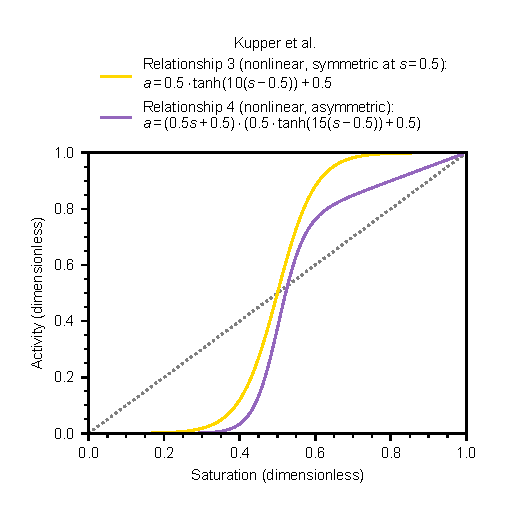
\includegraphics[scale=1.0]{figures/percolation.eps}
    \caption{Activity-saturation relationships describing percolation-limited electrolyte dry-out adapted from Figure 5 of Kupper et al.\cite{kupper_end--life_2018} Relationships 3 and 4 model percolation of the liquid electrolyte where activity depends nonlinearly on saturation. The key feature of both relationships is the presence of a percolation threshold value ($s=0.5$), around which activity varies rapidly between $0$ and $1$.
    The sensitivity of activity to small changes in saturation is apparent.}
    \label{fig:percolation}
\end{figure}

\subsection{Mechanical degradation knees}

Both microscale mechanical effects occurring at the particle scale and macroscale mechanical effects occurring at the cell scale are pathways for knees. 
While we have already discussed how mechanical degradation mechanisms can cause knees (e.g., loss of active material from delamination causing lithium plating), here we focus on knees more explicitly linked to mechanical effects.

\begin{figure}[ht]
\centering
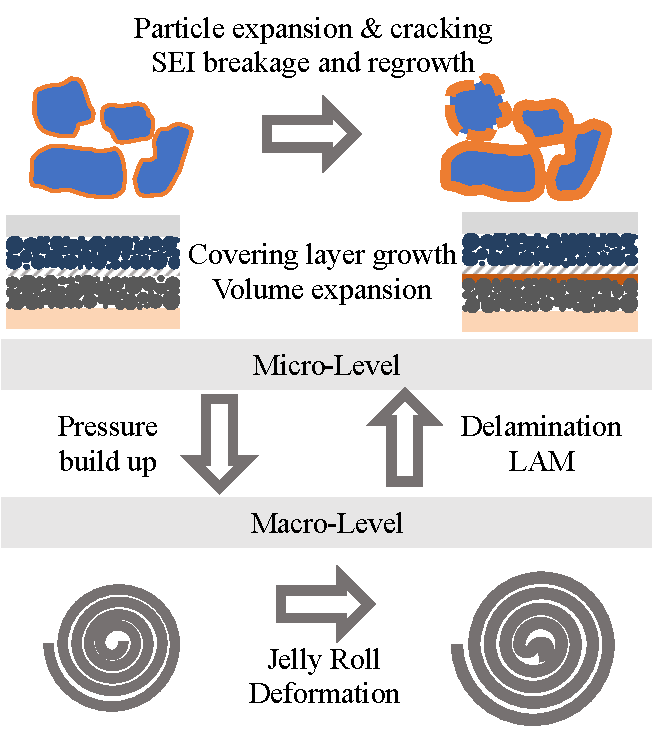
\includegraphics[scale = 1]{figures/MechanicalKneepoints.pdf}
\caption{Mechanical effects leading to Knee points: During cycling particles and the SEI expand and crack leading to the formation and regrowth of additional SEI. In addition a covering layer was found forming on the anode surface. Pressure due to volume expansion can also lead to jelly roll deformation in cylindrical wound cells. This can induce delamaniation and loss of active material leading to more SEI and covering layer growth.}
\label{fig:knee_mechanical}
\end{figure}

\paragraph{Micro scale mechanical effects.}

At the micro scale, repeated intercalation/de-intercalation causes stress in the particles that can then lead to loss of active material through particle cracking.
Reniers et al.~\cite{reniers_review_2019} showed that there can be a positive feedback between the stress and the loss of active material leading to a (snowballing) knee point. They model this using a fatigue model for loss of active material due to stress from Laresgoiti et al.~\cite{laresgoiti_modeling_2015} with a stress model from Dai et al.~\cite{dai_simulation_2014}: higher stress causes higher LAM, which in turn increases the current density and hence causes higher stress.

Other authors have suggested that mechanical effects can accelerate SEI growth by causing SEI cracking and revealing new active surface area to grow \cite{kupper_end--life_2018,louli_operando_2019}. Since SEI formation is still self-limiting, this effect alone is not enough to lead to a knee point, but it could accelerate the onset of knee points in other mechanisms related to SEI formation.
In addition to SEI formation, covering layers on the anode surface were reported on cells with knee points as shown in Figure~\ref{fig:covering_layers} \cite{lewerenz_post-mortem_2017,willenberg_development_2020,stiaszny_electrochemical_2014}. These layers were also characterized as passivating or dead lithium agglomerates \cite{schindler_fast_2018}.


\paragraph{Macro scale mechanical effects.}

High stack pressure, for example originating from micro scale effects, can cause knee points due to mechanical stress at the macro scale. Shown by Cannarella et al.~\cite{cannarella_stress_2014} high mechanical stress is not evenly distributed throughout the inside of the pouch, causing heterogeneous delamination, surface film formation, and uneven lithium distribution. Furthermore LAM attributed to anode from half-cell data, shows no change postive electrode active material. Similar to temperature there is a sweet spot for stack pressure\cite{cannarella_stress_2014}. 

For pouch cells \cite{wunsch_investigation_2019} and prismatic cells\cite{cannarella_stress_2014} bracing can be added to increase the lifetime, so the pressure over the lifetime evolves differently. Wünsch et al. \cite{wunsch_investigation_2019} reported a thickness increase for unbraced cells correlated with knee points. They also showed with the right bracing, for example deforming elements on both sides of the cells, the lifetime could be increased from 500 to 3200 cycles. For cylindrical cells\cite{willenberg_high-precision_2020} the pressure evolution can only be measured. From post-mortem analysis Bach et al. could show a link between heterogeneous pressure and uneven aging and plating\cite{bach_nonlinear_2016}.
In addition with CT studies by  Pfrang et al.~\cite{pfrang_long-term_2018} revealed jelly roll deformation in 18650s, using cells from Ecker et al. \cite{ecker_calendar_2014}

\subsection{Interactions and heterogeneity}

\pbox{This will be a new section discussing how everything's really complicated}

\section{Factors influencing the knee}

We surveyed the literature to identify empirical case studies in which the knee point can be controlled via changes to a single variable. Table S1 classifies these case studies into three categories based on the nature of the variable: cell design, testing conditions, and sampling/testing variability (a special case of these two categories). Some testing conditions have a consistent impact on the emergence of the knee; for example, higher charging rates and wider cycling voltage ranges accelerate the appearance of the knee. However, the impact of other variables (e.g., discharging rate and rest times) is less clear and may depend on the specific cell design and operating conditions.

\subsection{Cell design}

While the dependence of knees on cell usage conditions has been studied extensively, less attention has been focused on the dependence of knees on cell design---likely due to the challenges of lab-scale cell fabrication. Ma et al.\cite{ma_editors_2019}, one of the most comprehensive works on this topic, studied the impact of various electrodes and electrolytes on the location of the knee, finding that cathode particle coatings and low cathode loadings delayed the knee. These knees were classified as resistance ``pseudo-knees'' due to increased electrolyte oxidation on the cathode, as evidenced by the strong dependence of the knee severity on discharge rate as well as cathode impedance measurements. Ma et al. al.\cite{ma_editors_2019} and Glazier et al.\cite{glazier_analysis_2017} also found that the graphite type (i.e., natural or artificial) substantially impacts the knee location, though the root cause of the knee in this case is unclear(PETER TO EXPLORE FURTHER).

Electrode loadings---specifically, anode loadings---can also lead to knees via the lithium plating pathway.
If the electrode is too thin or the capacity is too low, thermodynamic plating can occur; however, kinetic plating can occur if the electrode is too thick. (LI PLATING TEAM--WHAT ARE GOOD REFERENCES FOR THESE?)

Additionally, small changes in the electrolyte can play an outsized role on the lifetime performance. Ma et al.\cite{ma_editors_2019} demonstrated the sensitivity of the knee location to the electrolyte additive package; specifically, high methyl acetate (MA) concentrations (MA is used to increase electrolyte transport capability) and low LiPF$_6$ concentrations consistently lead to earlier knees. These knees were attributed to increased electrolyte oxidation on the cathode. Ma et al.\cite{ma_editors_2019} also identified other electrolyte systems with a strong knee sensitivity. Additionally, as previously discussed, additive depletion (e.g., FEC depletion in cells with high silicon content in the anode) can be a direct cause of knees for some cell designs.

Lastly, mechanical deformation knees are naturally highly sensitive to the cell form factor. For instance, deformation of the core(PHILIPP -- WHAT PAPERS TO CITE?) can only occur in cells with cores, namely cylindrical cells.

\subsection{Testing conditions}

\subsubsection{Charging rate}
Increasing the charging rate has accelerated the onset of the knee-point across a range of batteries. \cite{lewerenz_systematic_2017,lewerenz_post-mortem_2017, petzl_lithium_2015, burns_-situ_2015, waldmann_optimization_2015, schuster_nonlinear_2015, severson_data-driven_2019, schindler_fast_2018, keil_linear_2019}. However, the critical charging rate leading to knee-onset varies substantially, with knees appearing at C-rates as low as 1C \cite{waldmann_optimization_2015} and as high as 8C \cite{lewerenz_systematic_2017}. 

Higher charging rates advance the knee point via Li plating and accelerated SEI growth. Either Li plating or SEI growth may directly cause knee onset, but knee onset is also attributed to pore clogging caused by either or both of these mechanisms \cite{yang_modeling_2017}. It is difficult to distinguish these causes, even in cases with detailed post-mortem characterization. Key evidence for both Li plating and accelerated SEI growth driven by increased charging rate is found in a series of papers by Lewerenz et. al., examining the aging of cylindrical 8 Ah LFP/Gr cells \cite{lewerenz_systematic_2017,lewerenz_post-mortem_2017}. They present evidence demonstrating that knees reliably occur across a set of test replicates at 8C charging rate, while knees may occur less reliably at charging rates as low as 2C. Evidence of Li plating after knee onset driven by increased charging rate was also confirmed by Petzl et. al. \cite{petzl_lithium_2015} and Burns et. al. \cite{burns_-situ_2015}. 



\subsubsection{Discharging rate}

Unlike charging rate, the effect of discharging rate on the knee point is mixed (Figure X).
In some systems, an increased discharging rate
accelerates the knee onset.
Omar et al.\cite{omar_lithium_2014} found that a higher discharging rate (1C to 15C) accelerated the knee for cylindrical LFP/graphite cells.
Diao et al.\cite{diao_accelerated_2019} showed no effect of discharge rate except at 60°C, where the cells discharged at 2C degraded almost twice as quickly as the cells discharged at 0.7C or 1C.
High discharging rates can lead to worse cycle life due to higher temperatures, which accelerates electrolyte reduction (i.e., SEI growth) and electrolyte oxidation (i.e., cathode resistance growth). Additionally, high discharging rates can lead to ``pseudo-knees'' when the resistance growth or lower cutoff voltage is high.

In other systems, an increased discharging rate can delay the onset of the knee.
Atalay et al.\cite{atalay_theory_2020} found that reducing the discharge rate from 4C to 1C accelerated the knee for 18650 NCA/graphite cells.
Keil et al.\cite{keil_charging_2016} illustrated how discharging current had no effect on LMO+NMC/graphite and LMO+LCO/graphite cylindrical cells, but a lower discharging current (3A, 2.7C) led to faster degradation than a higher discharging current (5A, 4.5C) for an LFP/graphite cylindrical cell when charged at 4.5C; they did not identify a mechanism. 
Similarly, Keil et al.\cite{keil_linear_2019} found that increasing discharging current from 1C to 2C led to the elimination of the knee in NMC/graphite cylindrical cells.
While more work is needed to understand these results, one hypothesis for these observations is decreased calendar aging for cells with faster discharge rates.
In other words, cells with less time spent cycling simply have less calendar aging. This hypothesis does suggest a sensitivity of the x axis to the apparent severity of the knee; for instance, plotting capacity retention vs. time instead of cycle number may decrease the apparent severity of the knee.

\subsubsection{Voltage limits} 
A wider voltage window generally accelerates the onset of the knee point \cite{ecker_calendar_2014, pfrang_long-term_2018, klett_non-uniform_2014, ma_novel_2019, petzl_lithium_2015, schuster_nonlinear_2015}. In one of the broadest studies, Ecker et al. \cite{ecker_calendar_2014} considered six DODs (100, 80, 50, 20, 10, and 0.5 \%) with up to six voltage windows per DOD. They found that the EFC systematically decreased with increased DOD. By 1000 EFC, all cells with DODs greater than 25-75 \% had a capacity below 80 \% and showed a knee point. When varying the voltage window at the same DOD, the authors observed the highest degradation in cells cycled at low and high SOCs; the lowest degradation was observed for a midpoint SOC of 50 \%. Accelerated degradation at extreme SOCs was also observed in other studies \cite{aiken_accelerated_2020,ma_novel_2019, zhu_investigation_2021}.

The impact of the voltage window on knee point onset is typically attributed to resistance growth stemming from enhanced expansion and cracking of the electrode during intercalation. In several studies, capacity knees have aligned perfectly with resistance knees \cite{ecker_calendar_2014, klett_non-uniform_2014, schuster_nonlinear_2015, zhu_investigation_2021}. High voltages may also drive electrolyte oxidation at the cathode \cite{aiken_accelerated_2020} and for some cathodes, active material loss via Mn dissolution \cite{ma_novel_2019}. 



\subsubsection{Rests}

The effect of rests during cycling on the knee occurrence is mixed. 
Keil et al.\cite{keil_linear_2019} found that decreasing rest time at both the top of charge and the bottom of discharge from 900 seconds to 10 seconds delayed the knee point in graphite/NMC cylindrical cells.
Ma et al.\cite{ma_editors_2019} found an identical result: removing the 30-minute rests at both top-of-charge and bottom-of-discharge delayed the knee, but only with an upper cutoff voltage of 4.3 V. The rest time had no effect at 4.1 V.
These observations were rationalized by less time at high potential when plotted as a function of cycle number.
In contrast, Epding et al.\cite{epding_investigation_2019} found that longer rest times between cycles delayed the knee occurrence. The authors proposed that this rest offered reversibly plated lithium time to reintercalate; another possibility is that the rest allowed for greater utilization of cycleable lithium(cite Rashid Gupta, see comment). More generally, increased rest periods may delay the onset of knees driven by high overpotentials (e.g., kinetic lithium plating at high rates or low temperatures) but may exacerbate the onset of knees driven by side reaction product buildup (e.g., porosity decrease, cathode resistance growth, etc)---particular for rests at high state of charge. In general, more work is needed to understand the sensitivity of knees to rest at both low and high state of charge.


\begin{figure}[ht]
\centering
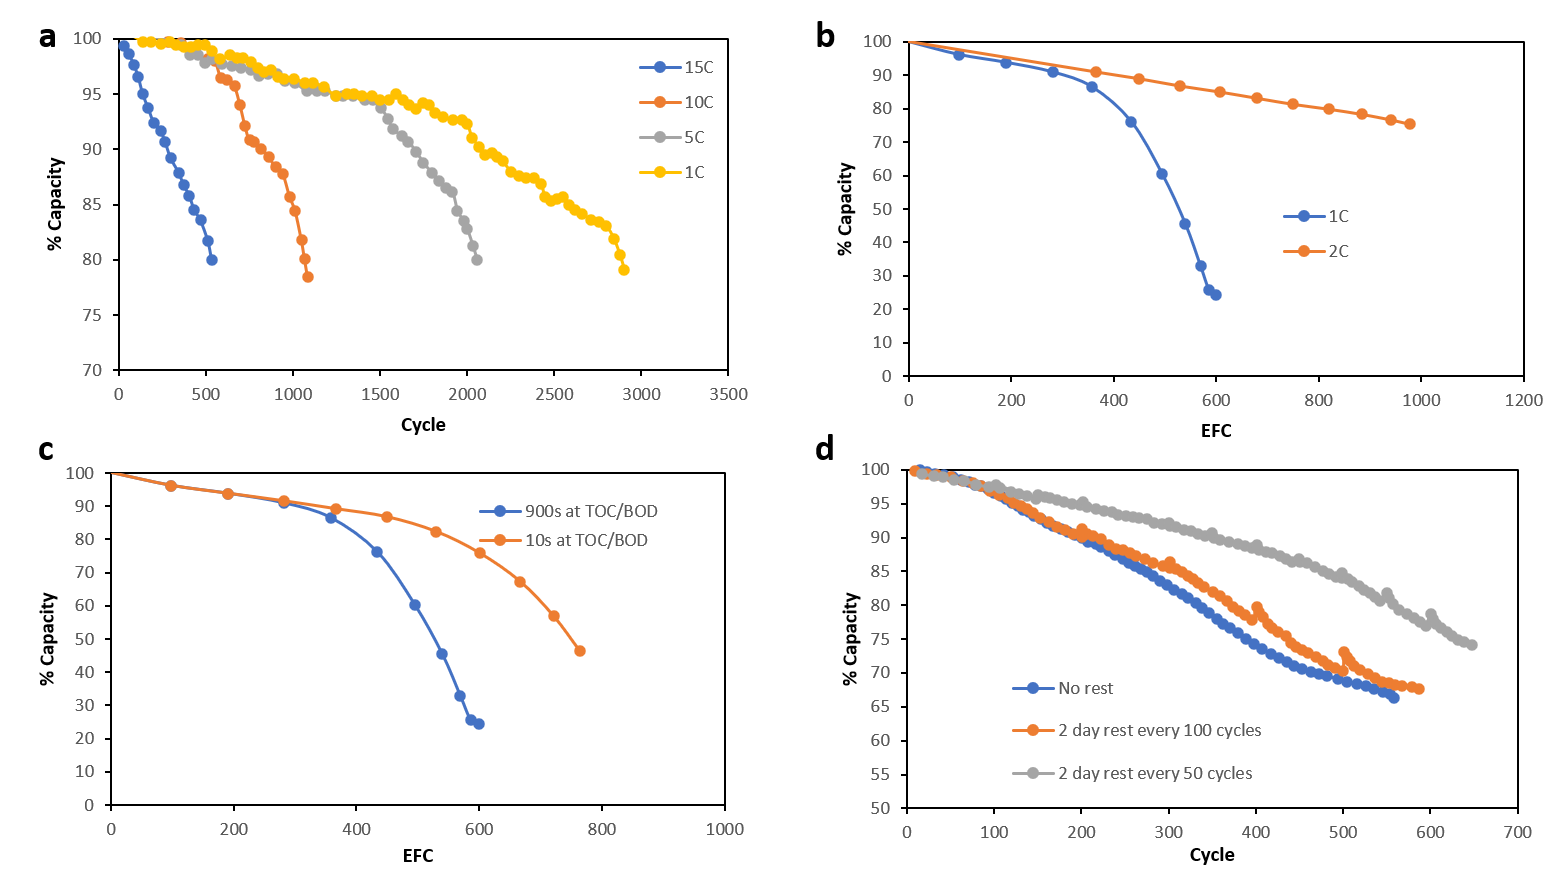
\includegraphics[scale = 1.0]{figures/Discharge-rest_cycle.png}
\caption{Discharge rate and rest time have mixed effects on knee point onset depending on the testing conditions. (a) Higher discharge rate accelerates knee onset. Adapted from \cite{omar_lithium_2014} (b) Lower discharge rate accelerates knee onset. Adapted from \cite{keil_linear_2019} (c) Longer rest time accelerates knee onset. Adapted from \cite{keil_linear_2019} (d) Shorter rest time accelerates knee onset. Adapted from \cite{epding_investigation_2019}. To isolate the influence of calendar aging, the above are replotted with a time axis in the Supporting Information.  }
\label{fig:discharge-rest_cycle}
\end{figure}


\subsubsection{Temperature}
The effect of temperature on knee onset depends on the test conditions. For example, some studies have found that knee onset is accelerated at temperatures above or below 25 degrees Celsius \cite{zhang_accelerated_2019, waldmann_temperature_2014, waldmann_optimization_2015} or 35 degrees Celsius \cite{schuster_nonlinear_2015}. In general, the temperature of minimal degradation is lower for LFP cells than NMC cells \cite{preger_degradation_2020}. 

There is no straightforward dependence on temperature because different mechanisms dominate in different temperature ranges (Figure \ref{fig:temperature_and_pressure}). At lower temperatures, the acceleration of the knee point is attributed to Li plating. At elevated temperatures, knee point onset is driven by SEI growth \cite {zhang_accelerated_2019,schuster_nonlinear_2015,waldmann_temperature_2014,waldmann_optimization_2015}.

\subsubsection{Pressure}
Studies of pressure dependence in pouch and prismatic cells have demonstrated 'sweet spots' for optimal performance. The knee point can be accelerated by either an absence of pressure or excess pressure. For example, Wünsch et al. increased the cycle life of 37 Ah commercial NMC pouch cells from 500 (no bracing) to 3200 (optimal spring compression) while investigating various methods of bracing \cite{wunsch_investigation_2019}. Figure \ref{fig:temperature_and_pressure} shows another example from Cannarella et al. for an LCO pouch cell \cite{cannarella_stress_2014}. Even in a cylindrical cell, heterogeneous compression in the test fixture can accelerate the knee point \cite{bach_nonlinear_2016}. 

For pouch and prismatic cells, some applied pressure is needed to enhance conductivity and particle contact. When too much pressure is applied, high mechanical stress is not always evenly distributed throughout the cell. This causes heterogeneous delamination, surface film formation, and uneven Li distribution (Li plating). Li plating was also reported in cylindrical cells that experienced heterogeneous compression from test fixtures \cite{bach_nonlinear_2016}. 

\begin{figure}[ht]
\centering
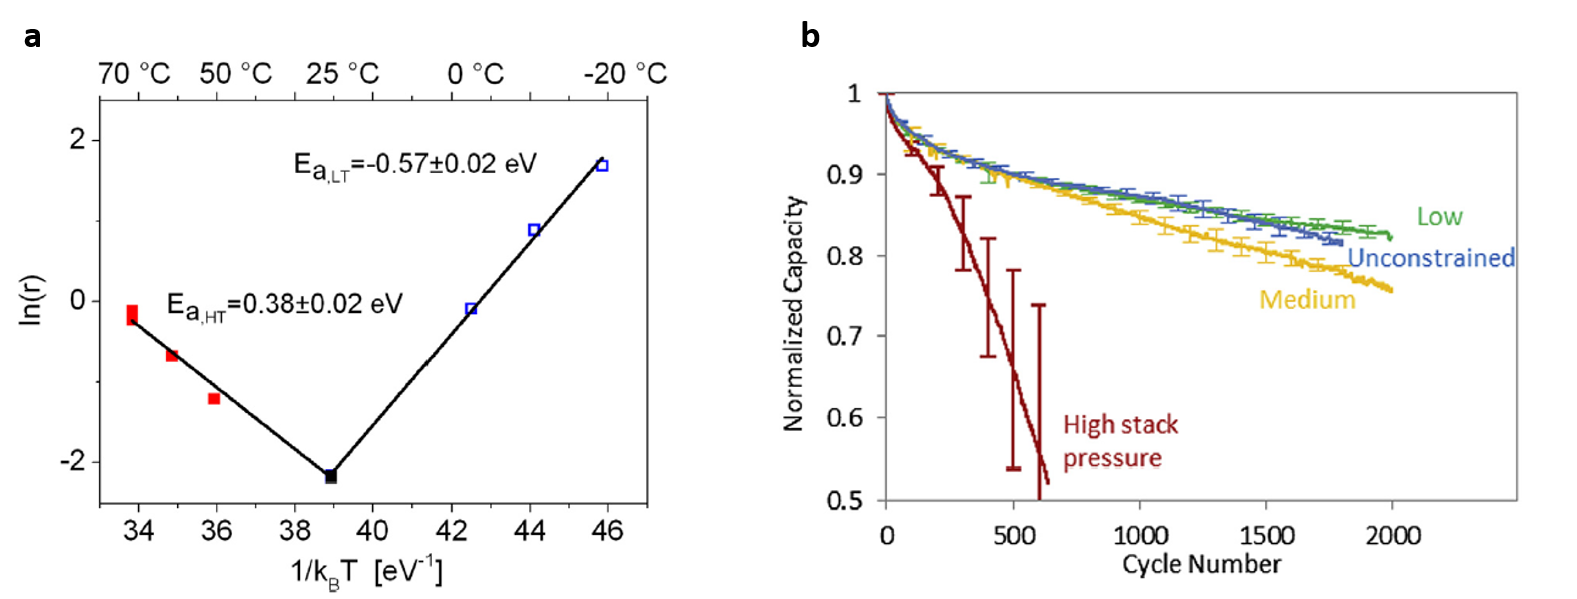
\includegraphics[scale = 1.0]{images/Temperature_and_pressure.png}
\caption{Transition in degradation mechanism based on (a) temperature and (b) applied pressure, illustrating a ``sweet spot'' for each variable. Adapted from Waldman et al.\cite{waldmann_temperature_2014} and Cannarella et al.\cite{cannarella_stress_2014}, respectively.}
\label{fig:temperature_and_pressure}
\end{figure}



\subsection{Sampling and testing variability}

Nominally identical cells cycled identically often show differences in knee behavior. This sampling variability includes both intrinsic variability from manufacturing (component-level variation, cell assembly, etc.) and extrinsic variability from testing (cycler calibration, temperature control, etc.). These sources of variability cannot be distinguished.

The magnitude of sampling variability is a function of the cell design, manufacturing variability, and testing conditions. Sampling variability may increase with more aggressive cell designs (e.g., higher silicon content), more manual cell assembly processes, and more aggressive testing conditions (particularly for test setups with no or poor temperature control). The magnitude of sampling variability can be estimated using studies with fairly large sample sizes (i.e., at least $\sim$10 cells). Baumhöfer et al.\cite{baumhofer_production_2014} and Harris et al.\cite{harris_failure_2017} studied this type of variation in 48 cells and 24 cells, respectively, finding widely varying knee locations across their datasets. These studies did not identify a correlation between beginning-of-life capacity and end-of-life capacity, suggesting that the underlying state variables controlling the knee location did not manifest in the initial capacity measurements. In general, sampling and testing variation also pose challenges for accurate knee prediction; we recommend identifying the manufacturing and testing variation of the state variable of interest in evaluating the accuracy of knee prediction methods. Beck et al.\cite{beck_inhomogeneities_2021} provide a detailed review of cell-to-cell variation.

\section{Modeling and predicting knees}

\pbox{Anyone interested? I think a key message here is which pathways/types of pathways can be predicted theoretically and with measurements}
\newline
\ssri{I think this would be really valuable because predicting knees is really the economic value addition from all the knee point analysis. We spoke a little bit about how ML could predict knees -- given how much we've talked about pathways (also as mentioned by Peter above), I think there is a point to be made about physics-inspired/physics informed ML i.e., an ML framework coupled with an electrochem model which is one of the few ways in which something about the pathways can also be said in addition to the ML predicted knee. Goes a long way in making falsifiable ML models wrt knees.}


Recently, joint prediction of capacity and internal resistance  trajectory degradation for was carried out in \cite{strange_prediction_2021}

\subsection{Empirical relationship between knees and end-of-life}

While predicting knees is important, predicting end-of-life is more directly relevant for product performance and estimating warranty costs. Thus, we explored empirically the linear relationship between knee locations and end-of-life across 15 datasets (306 cells) -- \gbox{refer to Yulia's table}. 

\begin{figure}[ht]
\centering
% \begin{subfigure}{.5\textwidth}
%   \centering
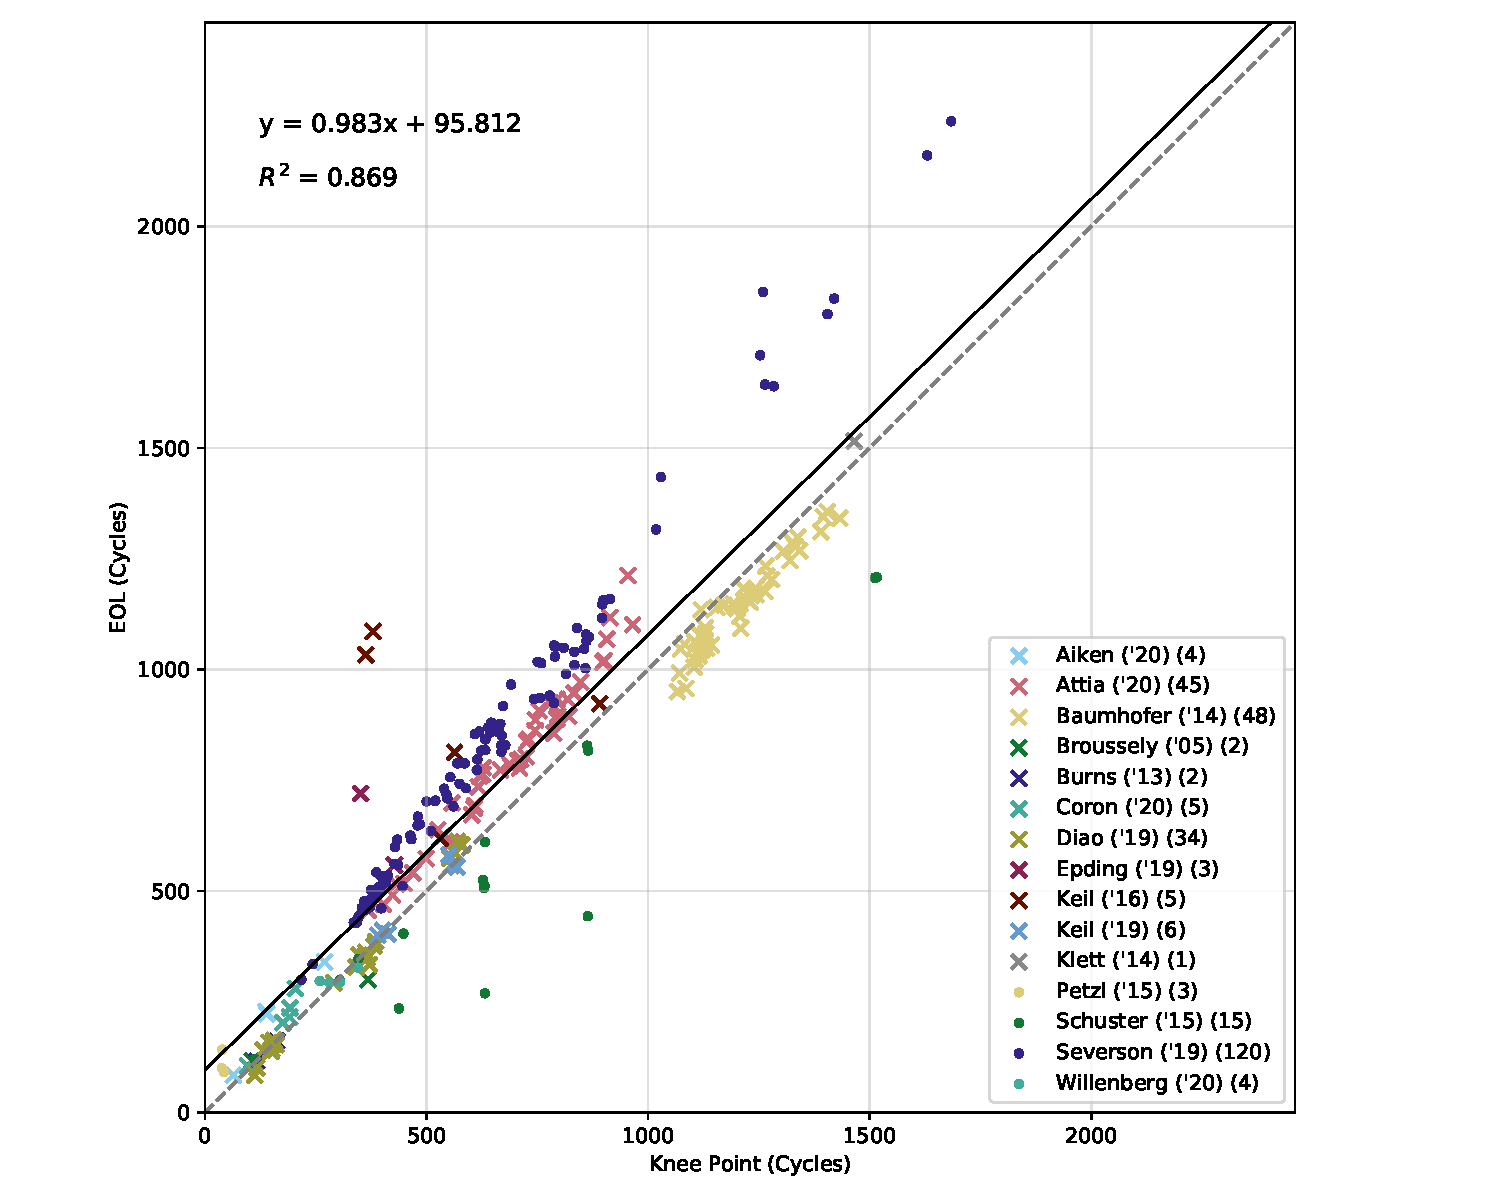
\includegraphics[scale=1.0]{figures/AcrossDatasetsknee-to-EOL}
%   \caption{Linear regression of knee-point to EOL point}
  \label{fig:kneepoint2EOL}
% \end{subfigure}%
\caption{Total of 306 cells across 15 datasets. The knee identification algorithm employed is the Bacon-Watts one. Linear relation between knee-point and EOL (defined as 80\% capacity).}
\label{fig:knees2EOL}
\end{figure}

\subsection{Modeling approaches}

The effects discussed here are inherently multidimensional (at the macro scale) in nature and hence cannot be captured by standard electrochemical models, which are one-dimensional at the macro scale. Instead, they would require complex three-dimensional models, whose computational complexity is prohibitively high for simulating degradation over hundreds of cycles. We are not aware of any current modeling efforts in this direction [right?]. One reduced-order modeling approach could be to couple one-dimensional electrochemical models with network models for the jellyroll \cite{tranter_probing_2020}. Another possible modeling approach is to use homogenization methods on the jellyroll \cite{psaltis_homogenisation_2020} to elucidate the mechanical behavior (and buckling) of the spirally-wound layers.

\subsection{Prediction outlook}

Figure \ref{fig:snowball_vs_hidden_vs_threshold} illustrates three types of underlying mechanisms.

\pbox{
Notes:
\begin{itemize}
    \item Prediction is very hard
    \item Explainable AI (with or without physics)--long term goal is to predict degradation from data. Clustering datasets based on pathways and training on each ("finding bananas in images"). Easier to design falsifiable hypotheses for knee point vs capacity fade trajectory
    \item Some are easier than others. For each mechanism
    \item Internal state estimation from past datasets -- then can simulate forward to extrapolate. Check if extrapolation matches data, continuously adjust. Snowballs/exponentials hard to extrapolate
\end{itemize}
}

Two takaways (yuliya)
1. What can we tell people immediately -- what can people to do today. 
- Decision tree (Form factor, high SOC, etc) schematic. Even answered negatively is useful.


2. Actionable items - better metrics or indicators for other mechanisms

Why resolve things at microscale if they can't be resolved at macroscale

\subsubsection{Prediction from lab data}


\subsubsection{Prediction in the field}
Online state estimation
Harder than the lab -- particle and electrode level effects
Active interrogation -- send in signals to identify state/parameters. Hard due to limited control

\pbox{My takeaways so far:
\begin{itemize}
    \item Snowballs will be hard to extrapolate
    \item Challenge is identifying the right state variable to track, and actually tracking it
    \item Some state variables are ``electrochemically invisible'', e.g. remaining FEC content in the electrolyte.
    \item Multiscale modeling needed (SEI growth/cathode resistance growth, electrode porosity/connnectivity changes, macroscale mechanical deformation)
    \item need for low rate cycling
    \item In the field vs lab testing
    \item Online estimation 
    \item Pulse measurements. Superlinear increase in resistance is bad news
\end{itemize}
}

Goncalo: Can the mechanism be predicted from the data?

\section{Conclusions and future work}

Knees are a major challenge to developing long-lasting lithium-ion batteries. In this work, we first evaluated definitions of knees and identified three different types of underlying mechanisms leading to a knee, each with different implications for knee prediction. We then critically investigated the literature support for (five/six) knee pathways, including lithium plating, resistance growth, additive depletion, percolation-limited connectivity, and mechanical deformation.

\section{Supporting Information}

Table S1. Summary of experimental variables leading to knee points


Yuliya: See table in Excel document tab 'SI-Exp Tables'. 

Table S2 classifies previous efforts to model the knee point as physics-based, equivalent circuit, or empirical. [add explanation of table columns]

Table S2. Summary of previous knee point modeling efforts

\section{Data and code availability}

All data and code are publicly available in the associated Zenodo repository(CITE) and on GitHub (https://github.com/tinosulzer/kneepoint-review).


\begin{figure}[ht]
\centering
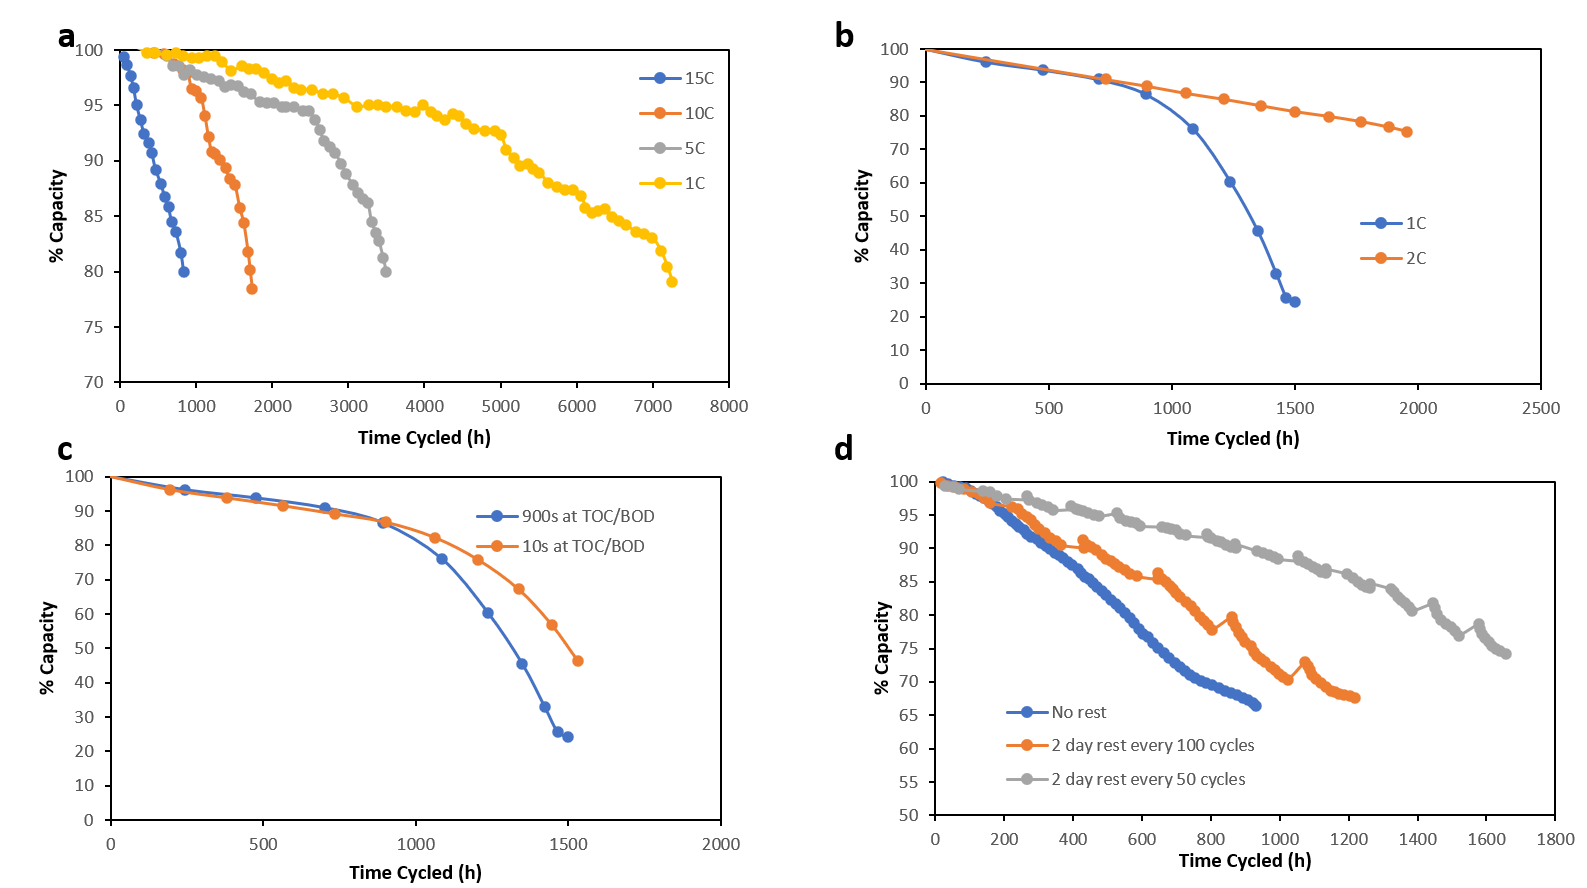
\includegraphics[scale = 1.0]{figures/Discharge-rest_time.png}
\caption{Discharge rate and rest time have mixed effects on knee point onset depending on the testing conditions. Data from Figure \ref{fig:discharge-rest_cycle} replotted with a time-based axis. (a) Higher discharge rate accelerates knee onset. Adapted from \cite{omar_lithium_2014} (b) Lower discharge rate accelerates knee onset. Adapted from \cite{keil_linear_2019} (c) Longer rest time accelerates knee onset. Adapted from \cite{keil_linear_2019} (d) Shorter rest time accelerates knee onset. Adapted from \cite{epding_investigation_2019}.}
\label{fig:discharge-rest_time}
\end{figure}

% \bibliographystyle{myIEEEtran}
\bibliography{refs_zotero}




\end{document}
